\documentclass[12pt,margin=0px]{article}

\usepackage[a4paper, margin=1in]{geometry}
\usepackage[export]{adjustbox}
\usepackage[hungarian]{babel}
\usepackage[normalem]{ulem}
\usepackage[table,xcdraw]{xcolor}
\usepackage[thinlines]{easytable}
\usepackage[utf8]{inputenc}
\usepackage{amsmath}
\usepackage{amssymb}
\usepackage{amsthm}
\usepackage{enumitem}
\usepackage{fancyhdr}
\usepackage{float}
\usepackage{fontawesome}
\usepackage{geometry}
\usepackage{graphicx}
\usepackage{hhline}
\usepackage{ifthen}
\usepackage{listings}
\usepackage{makecell}
\usepackage{multirow}
\usepackage{newunicodechar}
\usepackage{pgf,tikz}
\usepackage{subcaption}
\usepackage{tipa}
\usepackage{wasysym}
\usepackage{xcolor}

 \geometry{
 a4paper,
 total={170mm,257mm},
 left=20mm,
 right=20mm,
 top=20mm,
 bottom=20mm
 }

\definecolor{mygray}{rgb}{0.15, 0.15, 0.15}

\setlist[itemize,1]{label=$\bullet$}
\setlist[itemize,2]{label=$\circ$}
\setlist[itemize,3]{label=$\centerdot$}
\setlist[itemize,4]{label=$\cdot$}

\pagestyle{fancy}

\newcommand\blfootnote[1]{%
  \begingroup
  \renewcommand\thefootnote{}\footnote{#1}%
  \addtocounter{footnote}{-1}%
  \endgroup
}

\renewcommand{\figurename}{ábra}
\newenvironment{tetel}[1]{\paragraph{#1 \\}}{}

\newcommand\ddfrac[2]{\frac{\displaystyle #1}{\displaystyle #2}}

\newcommand{\N}{\mathbb{N}}
\newcommand{\Z}{\mathbb{Z}}
\newcommand{\R}{\mathbb{R}}
\newcommand{\Q}{\mathbb{Q}}
\newcommand{\C}{\mathbb{C}}

\makeatletter
\renewcommand\paragraph{%
	\@startsection{paragraph}{4}{0mm}%
	{-\baselineskip}%
	{.5\baselineskip}%
	{\normalfont\normalsize\bfseries}}
\makeatother

\useunder{\uline}{\ul}{}
\fancyhead{}
\cfoot{4. tétel | \thepage. oldal}

\renewcommand{\headrulewidth}{0pt}
\renewcommand{\footrulewidth}{0.4pt}

\begin{document}
    \thispagestyle{fancy}
    \hyphenation{oddword}
    \uchyph=0

    \begin{center}
        {\Large\bfseries\noindent 4. Számelmélet, gráfok, kódoláselmélet} \\
    \end{center}

    \section*{Számelmélet}

    \subsection*{Relációk, rendezések\\}
			
	\paragraph{Alapfogalmak}

    \begin{itemize}[leftmargin=5.5mm]
        \renewcommand{\labelitemi}{$\vcenter{\hbox{\tiny$\bullet$}}$}
        \item Az $(x,y)$ \emph{\textbf{rendezett pár}}, ha $(x,y) = (u,v) \Longleftrightarrow x = u \ \land \ y = v$.\\
        Ezt a tulajdonságot halmazokkal definiáljuk:
        \[
            (x,y) := \{ \{x\}, \{x, y\} \}
        \]
        \item Az $X,Y$ \textbf{\emph{halmazok Descartes-szorzata}} vagy direkt szorzata:
        \[
            X \times Y := \{ (x,y) : x \in X, y \in Y \}
        \]
        \item Ha $X, Y$ halmazokra $R \subset X\times Y$, akkor $R$ \emph{\textbf{reláció}} $X$ és $Y$ között.
        \item Egy halmazt \emph{\textbf{binér relációnak}} nevezünk, ha minden eleme rendezett pár.\\
        	Ha $R$ binér reláció és $(x,y) \in R$, akkor használható a következő jelölés: $xRy$
        \item Az $R$ binér reláció \emph{\textbf{értelmezési tartománya}}: $\textrm{dmn}(R) := \{ x\  | \ \exists y : (x,y)\in R  \}$
        \item Az $R$ binér reláció \emph{\textbf{értékkészlete}}: $\textrm{rng}(R) := \{ y\  | \ \exists x : (x,y)\in R  \}$
        \item Egy $R$ binér reláció \emph{\textbf{inverze}}: $R^{-1} := \{(a,b) : (b,a) \in R\}$
        \item Legyen $R$ binér reláció, és $A$ halmaz. Az $A$ \emph{\textbf{halmaz képe}}: $R(A) := \{y \ | \ \exists x\in A: (x,y) \in R\}$
        \item Az $R$ és $S$ binér relációk \emph{\textbf{kompozíciója}}:
        \[
            R \circ S := \{ (x,y) \ | \ \exists z : (x,z) \in S \ \land \ (z,y) \in R \ \}
        \]
    \end{itemize}

    \paragraph*{Tulajdonságok\\}
    Az $R$ egy $X$-beli binér reláció (azaz $R \subset X\times X$), és $\forall x,y,z \in X$, ekkor a reláció \\

    \renewcommand{\arraystretch}{1.8}
    {\footnotesize
    \noindent \begin{tabular}{|l|l|}
        \hline
        \textit{\textbf{reflexív}}               & $(x,x)\in R$ \\ \hline
        \textit{\textbf{irreflexív}}             & $(x,x)\notin R$ \\ \hline
        \textit{\textbf{szimmetrikus}}           & $(x,y)\in R \Longrightarrow (y,x) \in R $ \\ \hline
        \textit{\textbf{antiszimmetrikus}}           & $(x,y)\in R \ \land \ (y,x) \in R \Longrightarrow x = y$ \\ \hline
        \textit{\textbf{szigorúan antiszimmetrikus}} & $(x,y)\in R \Longrightarrow (y,x) \notin R$ \\ \hline
        \textbf{tranzitív}           & $(x,y)\in R \ \land \ (y,z) \in R \Longrightarrow (x,z) \in R $ \\ \hline
        \textit{\textbf{trichotóm}}              &
        \begin{tabular}[c]{@{}l@{}}Ha minden $x,y \in X$ esetén az alábbiak közül pontosan egy teljesül\\
            $\quad \ a)\ x=y$\\
            $\quad \ b)\ (x,y) \in R$\\
            $\quad \ c)\ (y,x) \in R$\\
        \end{tabular} \\ \hline
        \textit{\textbf{dichotóm}}               & $(x,y) \in R \ \lor \ (y,x) \in R$ \\ \hline
        \end{tabular}
    }\\
    \renewcommand{\arraystretch}{1}

    \paragraph*{Rendezések}

    \noindent Legyen $X$ halmaz, $R$,$S$ relációk $X$-beliek.

    \begin{itemize}[leftmargin=5.5mm]
        \renewcommand{\labelitemi}{$\vcenter{\hbox{\tiny$\bullet$}}$}
        \item Az $R$ binér reláció \emph{\textbf{ekvivalenciareláció}}, ha
       	\begin{itemize}
            \renewcommand{\labelitemii}{$\vcenter{\hbox{\tiny$\triangleright$}}$}
        		\item Reflexív
        		\item Szimmetrikus
        		\item Tranzitív
        	\end{itemize}

        \item Az $R$ binér reláció \emph{\textbf{részbenrendezés}}, ha
        \begin{itemize}
            \renewcommand{\labelitemii}{$\vcenter{\hbox{\tiny$\triangleright$}}$}
        	\item Reflexív
        	\item Antiszimmetrikus
        	\item Tranzitív
        \end{itemize}

        \item Az $R$ binér reláció \emph{\textbf{(teljes) rendezés}}, ha
        \begin{itemize}
            \renewcommand{\labelitemii}{$\vcenter{\hbox{\tiny$\triangleright$}}$}
        	\item Részbenrendezés, és
        	\item Dichotóm
        \end{itemize}
%        \item $S$-et az $R$ \emph{szigorítás}ának nevezzük, ha
%        \[
%        (x,y) \in R \ \land \ x \neq y \Rightarrow (x,y) \in S
%        \]
%        \\
%        Megfordítva, ha
%        \[
%            (x,y) \in R \ \lor \ x = y \Rightarrow (x,y) \in T
%        \]
%        akkor $T$ az $R$-hez megfelelő \emph{gyenge reláció}.\\

        \item $X$ részhalmazainak egy $\mathcal{O}$ rendszerét \emph{\textbf{osztályozás}}nak hívjuk, ha $\mathcal{O}$ páronként diszjunkt nemüres halmazokból álló halmazrendszer, melyre $\bigcup\mathcal{O} = X$.\\

        \textbf{Tétel}: Egy ekvivalenciareláció meghatároz egy osztályozást.\\
        Fordítva: $\mathcal{O}$ osztályozásra, az $R = \bigcup\Big\{Y\times Y : Y \in \mathcal{O} \Big\}$ ekvivalenciareláció.

	\end{itemize}

    \subsection*{Korlátok\\}

        \paragraph*{Legkisebb, legnagyobb, minimális, maximális elem}
        $X$ halmazbeli \emph{részbenrendezés} ($\preccurlyeq$) \emph{legkisebb} (legelső) eleme egy olyan $x\in X$, hogy
            \[
                \forall y \in X : x\preccurlyeq y
            \]
            (Ilyen nem biztos, hogy létezik, de ha igen, akkor egyértelmű).\\
        $X$ halmazbeli \emph{részbenrendezés} ($\preccurlyeq$) \emph{legnagyobb} (utolsó) eleme egy olyan $x\in X$, hogy
            \[
                \forall y \in X : y \preccurlyeq x
            \]
            \begin{itemize}
                \renewcommand{\labelitemii}{$\vcenter{\hbox{\tiny$\triangleright$}}$}
                \item $x$-et \emph{\textbf{minimálisnak}} nevezzük, ha nincs nála kisebb elem,
                \item $x$-et \emph{\textbf{maximálisnak}} nevezzük, ha nincs nála nagyobb elem.
            \end{itemize}
            (Szemben a legkisebb/legnagyobb elemekkel, minimális/maximális elemből több is lehet.\\
            Ha viszont $X$ rendezett, akkor legkisebb=minimális, legnagyobb=maximális.)
        \paragraph*{Alsó, felső korlát}
        $X$ részbenrendezett halmaz, $Y \subset X$. Az $x \in X$ elem az $Y$
            \begin{itemize}
                \renewcommand{\labelitemii}{$\vcenter{\hbox{\tiny$\triangleright$}}$}
                \item \emph{alsó korlátja}, ha $\forall y \in Y : x \preccurlyeq y$.
                \item \emph{felső korlátja}, ha $\forall y \in Y : y \preccurlyeq x$.
            \end{itemize}
            Látható, hogy $x$ nem feltétlenül eleme $Y$-nak, sőt az is lehet, hogy $Y$-nak nincs alsó/felső korlátja, vagy akár több is van. Ha azonban $x\in Y$, akkor egyértelmű és ez Y legkisebb eleme.
        \paragraph*{Infimum, szuprémum}
        Ha az alsó korlátok között van \emph{legnagyobb elem}, azt $Y$ alsó határának, \emph{\textbf{infimum}}ának nevezzük. (Jelölése: $\inf Y$) \\
        Ha a felső korlátok között van \emph{legkisebb elem}, azt $Y$ felső határának, szuprémumának nevezzük. (Jelölése: $\sup Y$)
        \paragraph*{Alsó, felső határ tulajdonság}
        $X$ részbenrendezett halmaz. Ha $ \forall\ \emptyset \neq Y \subset X$ : $Y$ felülről korlátos és van \emph{\textbf{szuprémum}}a, akkor felső határ tulajdonságú.
        Illetve ha $ \forall\ \emptyset \neq Y \subset X$ : $Y$ alulról korlátos és van infimuma, akkor alsó határ tulajdonságú.

    \subsection*{Függvények és műveletek}

    \subsubsection*{Függvények}

        Egy $f$ reláció \emph{\textbf{függvény}}, ha
        \[
            (x,y) \in f \ \land (x,y') \ \in f \Longrightarrow y = y'
        \]
        Más szóval minden $x$-hez legfeljebb egy olyan $y$ létezik, hogy $(x,y) \in f$\\

        \noindent Így minden $x \in$ dmn($f$)-re az $f(x) = \{y\}$.\\
        \emph{Jelölése}: $f(x) = y$\ \ vagy\ \ $f: x \mapsto y$\ \ vagy\ \ $f_x = y$.

        \paragraph*{Értelmezési tartomány, értékkészlet\\}
        Az $f : X \rightarrow Y$ jelölést használjuk, ha dmn($f$) $ = X $. \\
        Az $f \in X \rightarrow Y$ jelölést használjuk, ha dmn($f$) $\subset X$ (amikor dmn($f$)$ \subsetneq X$ is előfordulhat).\\
        Mindkét esetben rng($f$) $\subset Y$.\\

        \noindent Az $f$ függvény\\

        \renewcommand{\arraystretch}{2}
          $\begin{array}{|c|c|c|}
            \hline
            \makecell{\text{\emph{\textbf{injektív}}}\\ \text{kölcsönösen egyértelmű}} & \emph{\textbf{szürjektív}} & \emph{\textbf{bijektív}} \\ \hline
            f(x) = y \ \land \ f(x') = y \ \Longrightarrow \ x = x' & \forall y \in Y : \exists x\in X : f(x) = y & \emph{injektív és szürjektív} \\
            \makecell{\text{Ez azzal ekvivalens, hogy}\\ f^{-1}\ \text{reláció is függvény.}} & \makecell{\text{Azaz}\ rng(f) = Y.\\ \text{Tehát az \emph{f} függvény}\\ \text{az egész \emph{Y}-ra képez.}} &  \\ \hline
        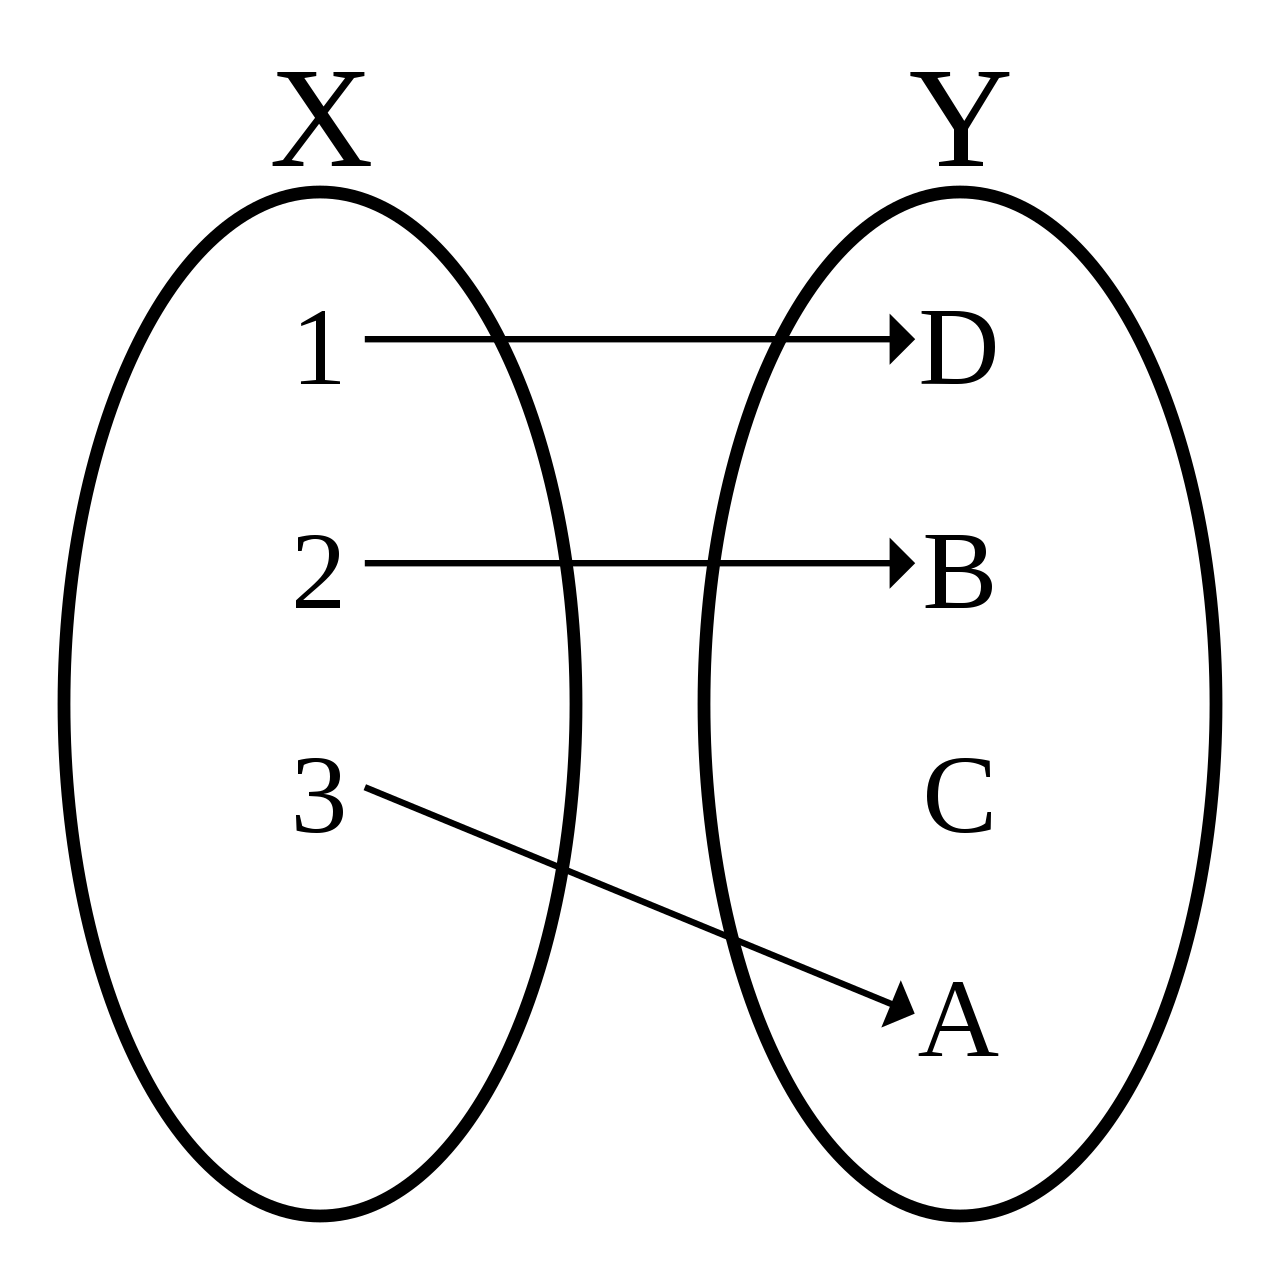
\includegraphics[width=0.25\textwidth]{img/injection.png}
        &
        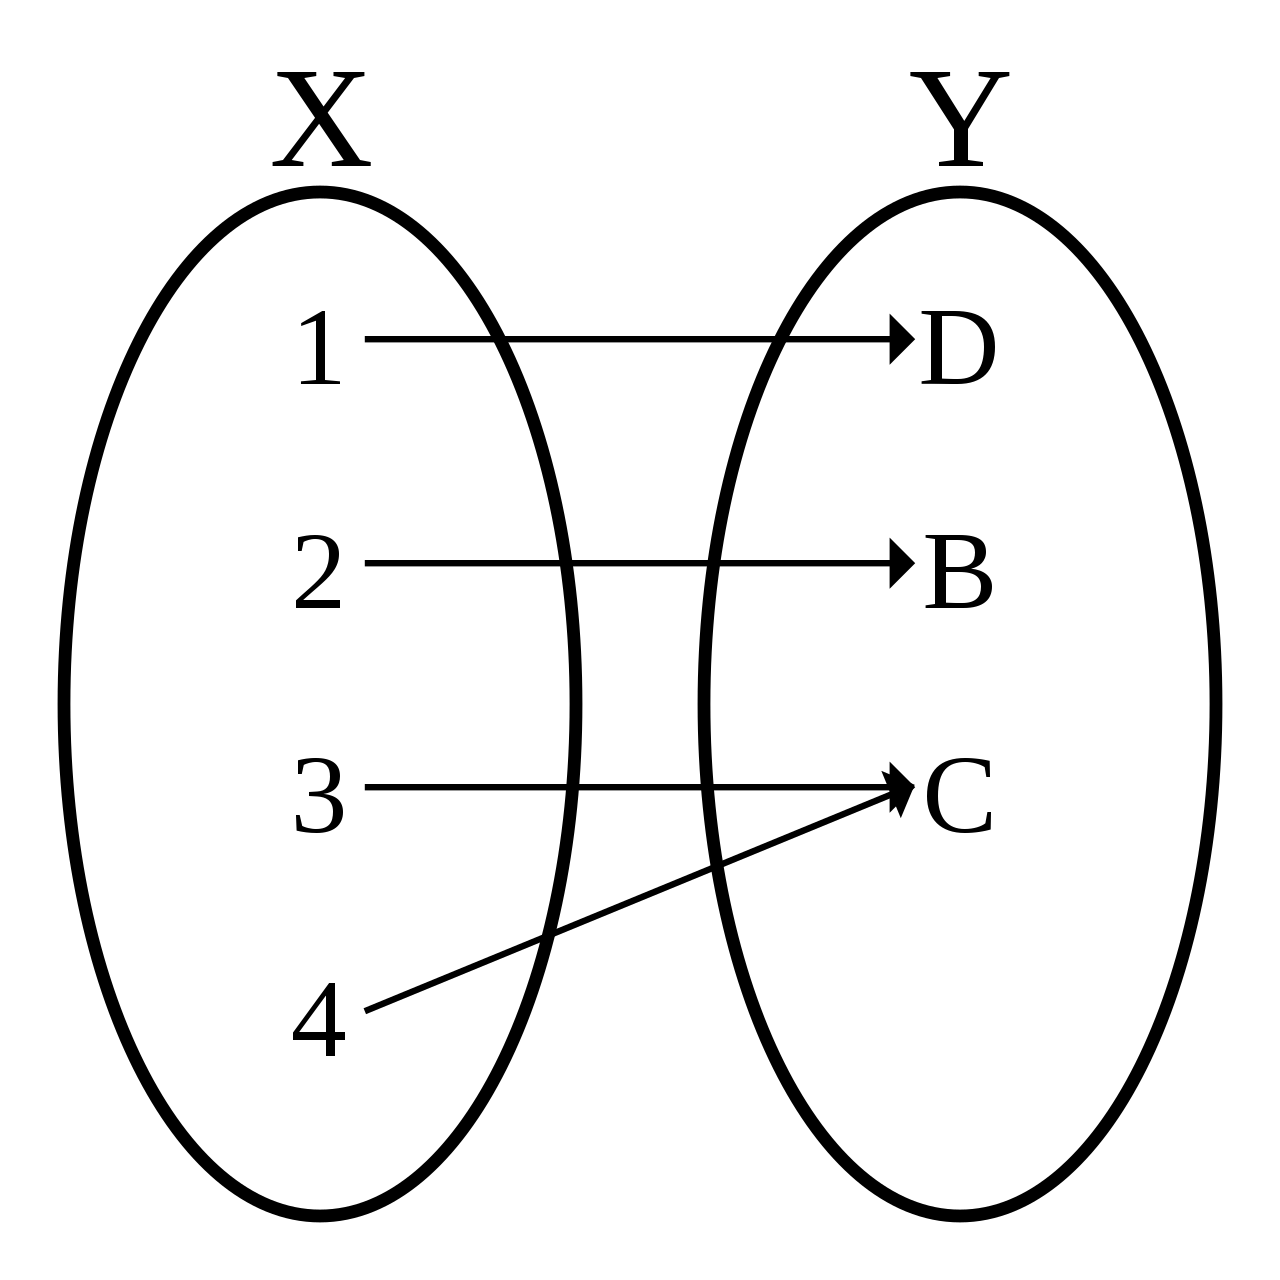
\includegraphics[width=0.25\textwidth]{img/surjection.png}
         &
        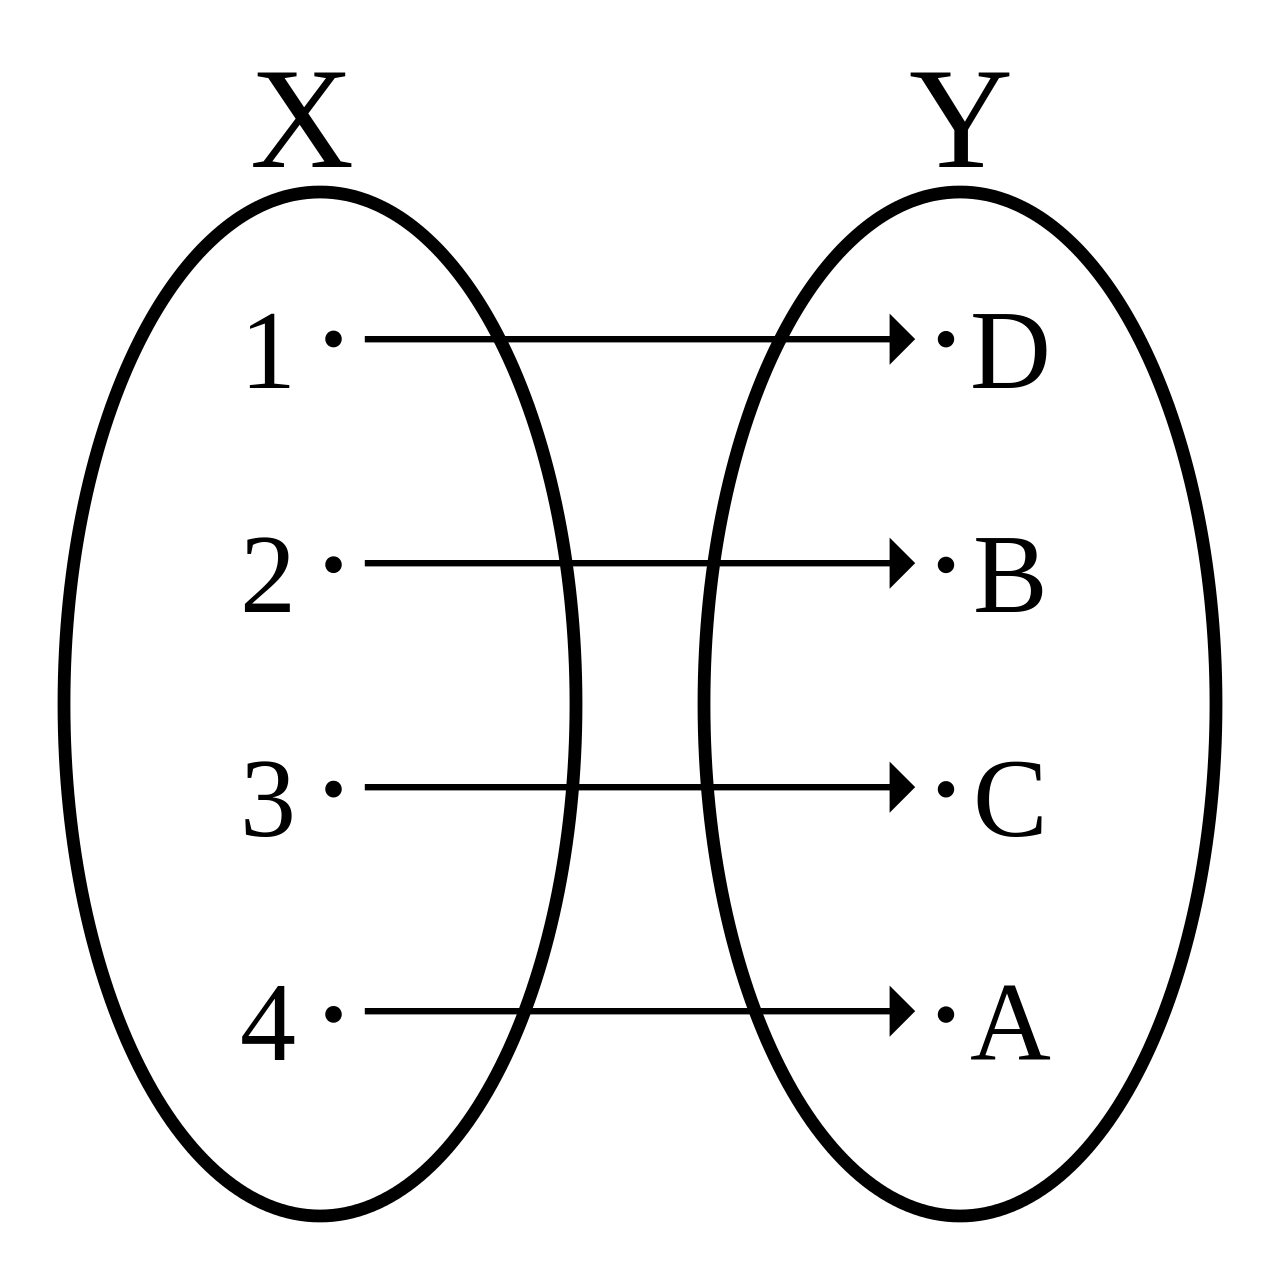
\includegraphics[width=0.25\textwidth]{img/bijection.png}
         \\ \hline
        \end{array}$
        \renewcommand{\arraystretch}{1}

        \paragraph*{Indexelt család\\}
        Az $x$ függvény $i$ helyen felvett értékét $x_i$-vel is szoktuk jelölni.\\

        \noindent Ilyenkor gyakran
        \begin{itemize}[leftmargin=5.5mm]
            \renewcommand{\labelitemi}{$\vcenter{\hbox{\tiny$\bullet$}}$}
            \item dmn($f$) = $I$ értelmezési tartományt \emph{\textbf{indexhalmaz}}nak, az
            \item elemeit \emph{\textbf{index}}eknek,
            \item rng($f$)-et \emph{\textbf{indexelt halmaz}}nak, és magát
            \item az $x$ függvényt \emph{\textbf{indexelt család}}nak szoktuk nevezni.
        \end{itemize}

		\subsection*{Műveletek}

        \begin{itemize}[leftmargin=5.5mm]
            \renewcommand{\labelitemi}{$\vcenter{\hbox{\tiny$\bullet$}}$}
            \item \textbf{Binér művelet}: $f : \textbf{X} \times \textbf{X} \rightarrow X$ függvény az $X$ halmazon.
            \item \textbf{Unér művelet}: $f : \textbf{X} \rightarrow X$ függvény az $X$ halmazon.
            \item \textbf{Nullér művelet}: $f : \{\emptyset \} \rightarrow X$ az $X$ halmazon. (Gyakorlatilag elemkiválasztás)
        \end{itemize}

        \paragraph*{Tulajdonságok}

        \begin{itemize}[leftmargin=5.5mm]
            \renewcommand{\labelitemi}{$\vcenter{\hbox{\tiny$\bullet$}}$}
            \item Legyen $\boxplus, \circledcirc$ binér műveletek $X$-en. $\forall x,y,z \in X.$
        	\begin{enumerate}
                \item $\boxplus$ \emph{\textbf{asszociatív}}, ha
                \[
                    (x \ \boxplus \ y ) \ \boxplus \ z = x \  \boxplus \  (y \ \boxplus z)
                \]
                \item $\boxplus$ \emph{\textbf{kommutatív}}, ha
                \[
                    x \ \boxplus \ y = y \  \boxplus \  x
                \]

                \item $\boxplus$ \emph{\textbf{disztributív}} a $\circledcirc$-ra, ha
                \[
                    x \  \boxplus \  (y \ \circledcirc \ z) = (x \  \boxplus \ y) \ \circledcirc \ (x \ \boxplus \ z) \quad \textrm{ - baloldali}
                \]
                \[
                    (y \ \circledcirc \ z) \  \boxplus \ x = (y \  \boxplus \ x) \ \circledcirc \ (z \ \boxplus \ x) \quad \textrm{ - jobboldali}
                \]
        	\end{enumerate}
        	
        \item Legyen $\circledcirc $ binér művelet $X$-en és $\boxdot$ binér művelet $Y$-on
        $f : X \rightarrow Y$ \emph{\textbf{művelettartó}} ha:
        \[ \forall x_1,x_2 \in X:  f(x_1 \ \circledcirc \ x_2) = f(x_1) \ \boxdot \ f(x_2) \]
        \end{itemize}

    \section*{Számfogalom, komplex számok}

    \subsection*{Számfogalom}

    \paragraph*{Algebrai struktúrák\\}

    \noindent Legyen $G$ halmaz és $\star$ egy művelet\\

        \noindent \emph{\textbf{Semleges (egység) elem}}: $a \in G$ semleges elem, ha $\forall g \in G : a \star g = g \star a = g$.\\

        \noindent \emph{\textbf{Inverz elem}}: $g,g^{-1} \in G$ és $a\in G$ semleges elem, akkor a $g^{-1}$ a $g$ inverze, ha
        \[
            g\star g^{-1} = a\ \text{és}\ g^{-1} \star g = a
        \]

        \noindent \emph{\textbf{Nullosztó}}: $x,y$ nullától különböző elemek, de $x\cdot y = 0$.
            (\emph{x} bal oldali, \emph{y} jobb oldali nullosztó)

        \begin{itemize}[leftmargin=5.5mm]
            \renewcommand{\labelitemi}{$\vcenter{\hbox{\tiny$\bullet$}}$}
            \item A	$G$ halmaz egy $\star$ művelettel, azaz a $(G, \star)$ párt \emph{\textbf{grupoid}}nak nevezzük.
            \item Ha egy grupoidban a $\star$ \emph{művelet asszociatív}, akkor a grupoid \emph{\textbf{félcsoport}}.
            \item \emph{Semleges elemes félcsoportot} \emph{\textbf{monoid}}nak nevezzük.
            \item Ha egy \emph{monoidban minden elemnek van inverze}, akkor \emph{\textbf{csoport}}ról beszélünk.
            \item Ha egy \emph{csoportban a művelet kommutatív}, akkor \emph{\textbf{Abel-csoport}}.
            \item Az $(R,+,\cdot)$ \emph{\textbf{gyűrű}}, ha
            \begin{itemize}
                \item az összeadással Abel-csoport,
                \item a szorzással félcsoport és
                \item teljesül mindkét oldali disztributivitás.
            \end{itemize}
            	
            Ha a \emph{szorzás kommutatív}, akkor \textbf{\emph{kommutatív gyűrű}}.
            	
            Ha a \emph{szorzásnak van egységeleme}, akkor \emph{\textbf{egységelemes gyűrű}}.
            \item A nullosztó mentes kommutatív gyűrűt \emph{\textbf{integritási tartomány}}nak nevezzük.
            	
            \item Az $R$ integritási tartomány \emph{\textbf{rendezett integritási tartomány}}, ha rendezett halmaz, továbbá az összeadás és szorzás monoton.
            	\begin{itemize}
            	\item \textit{Összeadás monoton: $x,y,z \in R$ és $x \leq y \ \Rightarrow \ x+z \leq y+z$
            	\item Szorzás monoton: $x,y \in R$ és $x,y\geq0 \ \Rightarrow \ x\cdot y \geq 0$ }
                    \end{itemize}
            \item Egy $R$ gyűrűt, ha $R\setminus\{0\}$ \emph{szorzással Abel-csoport}, akkor \emph{\textbf{test}}nek nevezzük.
            \item Ha egy test rendezett integritási tartomány, akkor \emph{\textbf{rendezett test}}.
        \end{itemize}

        \subsubsection*{Természetes számok}
                Legyen $^+ : \N \rightarrow \N$ unér művelet. Az alábbi feltételeket \emph{\textbf{Peano-axiómák}}nak nevezzük:
                \renewcommand{\arraystretch}{2}
                 $\begin{array}{ll}
                1.\ \ 0 \in \N & \text{(a 0 természetes szám)} \\
                2.\ \ \forall n \in \N, \exists! n^+ \in \N \textit{, hogy}\ n \neq n^+ & \text{(n \emph{rákövetkezője})} \\
                3.\ \ \nexists n \in \N,\ \text{hogy}\ n^+ = 0 & \makecell[l]{(\text{nem létezik olyan természetes szám,}\\ \text{aminek a 0 a rákövetkezője})} \\
                4.\ \ \text{Ha}\ n,\ m\ \in \N,\ \text{és}\ m^+ = n^+,\ akkor\ n = m & \text{(a $^+$ művelet injektív)} \\
                5.\ \ \makecell[l]{A \subseteq \N,\ 0 \in A,\ \text{továbbá}\\ \forall n \in A : n^+\in A,\ \text{akkor}\ A = \N} & \text{(a matematikai indukció elve)}
                  \end{array}$\\\\
                \renewcommand{\arraystretch}{1}

        \noindent \textbf{Tétel}. Van olyan $\big(\mathbb{N}, (0,^{+})\big)$ pár, amely eleget tesz a Peano axiómáknak.\\
\newpage
        \noindent \textbf{Műveletek}
        {\small
        \begin{itemize}[leftmargin=5.5mm]
        \renewcommand{\labelitemi}{$\vcenter{\hbox{\tiny$\bullet$}}$}
            \item Összeadás \\
            $k,m,n \in \N$, akkor:
            \begin{enumerate}
            \item \emph{Asszociatív}: $(k+m)+n = k+(m+n)$
            \item \emph{Kommutatív}: $n+k = k+n$
            \item $n+0 = 0+n = n \qquad$ \textit{(\textbf{0}: additív zéruselem)}
            \item \emph{Egyszerűsítési szabály}: $n+k = m+k$ vagy $k+n = k+m$, akkor $m=n$
            \end{enumerate}
            \item Szorzás \\
            $k,m,n \in \N$, akkor:
            \begin{enumerate}
            \item \emph{Asszociatív}: $(k\cdot m)\cdot n = k\cdot (m\cdot n)$
            \item \emph{Kommutatív}: $n\cdot k = k\cdot n$
            \item $ 0\cdot n = n\cdot 0 = 0 \qquad$ \textit{(\textbf{0}: multiplikatív zéruselem)}
            \item $n\cdot 1 = 1\cdot n = n \qquad$ \textit{(\textbf{1}: a multiplikatív egységelem)}
            \item \emph{Disztributív}: $k\cdot (m+n) = k\cdot m + \cdot n$, illetve $(m+n) \cdot k = m\cdot k+n\cdot k$
            \item \emph{Egyszerűsítési szabály}:  $k\neq 0$ esetén: $n\cdot k = m\cdot k$, akkor $m=n$
            \end{enumerate}
        \end{itemize}
        }

        \subsubsection*{Egész számok\\}
        Természetes számok körében az összeadásra nézve csak a nullának van inverze, másként szólva, a kivonás általában nem végezhető el.\\

        \noindent Tekintsük a $\sim\ \subset\mathbb{N}\times\mathbb{N}$ relációt. Értelmezzük ezeken a párokon a
        \begin{itemize}[leftmargin=5.5mm]
        \renewcommand{\labelitemi}{$\vcenter{\hbox{\tiny$\bullet$}}$}
            \item $(a,b) \sim (c,d)$ relációt, ha $a+d = c+b$ relációt, az
            \item $(a,b)+(c,d) = (a+c,b+d)$ összeadást, a
            \item $(a,b)\cdot(c+d) = (a \cdot c + b \cdot d, a \cdot d + c \cdot b)$ szorzást, valamint a
            \item $(a,b)\leq (c,d)$, relációt ha $a+d \leq c + b$
        \end{itemize}

        \noindent A $\sim$ ekvivalenciareláció. Az ekvivalenciaosztályok halmazát jelöljük $\mathbb{Z}$-vel. Az így nyert halmazt nevezzük az egész számok halmazának.\\

        \noindent Mindegyik ekvivalenciaosztály reprezentálható az $(n,0)$ vagy $(0,n)$ (vagy akár egyszerre mindkettő) alakú elemével. Az $n \in \mathbb{N}$ számot az $[(n,0)]$ osztály azonosítja (más szóval a természetes számok beágyazhatók $\mathbb{Z}$-be), illetve a $[(0,n)]$ osztályt $–n$-nel jelöljük (így megkaptuk az összes ekvivalenciaosztályt, a $[(0,0)]$ osztályt kétszer, hiszen $–0=0$).\\

        \noindent Így az $[(a,b)]$-t
            ${\displaystyle {\begin{cases}a-b,&{\mbox{ha }}a\geq b\\-(b-a),&{\mbox{ha }}a<b\end{cases}}}$
        módon jelölhetjük.\\

        \noindent Ez a jelölés az egész számok megszokott reprezentációját adja: $\{... –3, –2, –1, 0, 1, 2, 3, ...\}$.\\
\newpage
        \noindent \emph{Például}:

        ${\displaystyle {\begin{aligned}0&=[(0,0)]&=[(1,1)]&=\cdots &&=[(k,k)]\\1&=[(1,0)]&=[(2,1)]&=\cdots &&=[(k+1,k)]\\-1&=[(0,1)]&=[(1,2)]&=\cdots &&=[(k,k+1)]\\2&=[(2,0)]&=[(3,1)]&=\cdots &&=[(k+2,k)]\\-2&=[(0,2)]&=[(1,3)]&=\cdots &&=[(k,k+2)].\end{aligned}}}$\\

        \noindent $\mathbb{Z}$ elemei a szokásos műveletekkel \textbf{gyűrű}t alkotnak. Az $(a,b)$ pár additív inverze a $(b,a)$ pár.

        \noindent A piros pontok a természetes számok rendezett párjait mutatják. Az összekötött piros pontok a vonal végén kékkel írt egész számot reprezentáló ekvivalenciaosztályok.
        \begin{figure}[H]
            \centering
            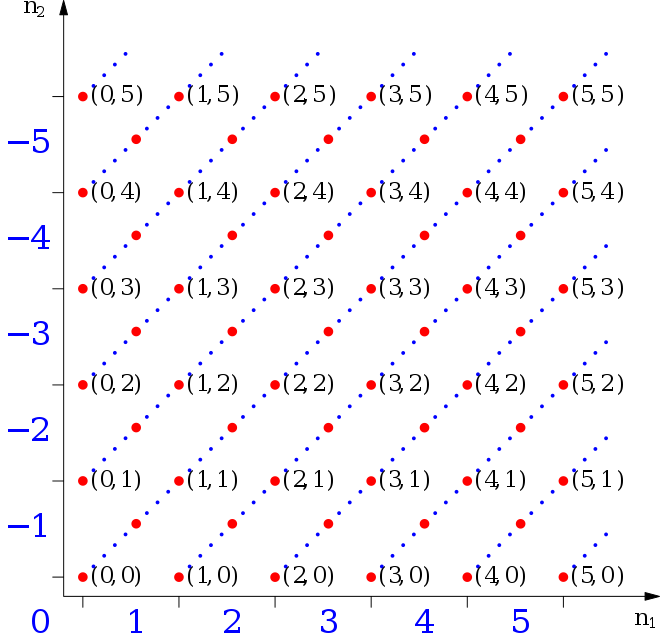
\includegraphics[width=0.35\textwidth]{img/660px-Relative_numbers_representation.svg.png}
            \label{fig:z}
        \end{figure}

    \subsubsection*{Racionális számok}
    Az egész számok körében a nem nulla elemek közül csak az 1-nek és a $-1$-nek van multiplikatív inverze, másként szólva az osztás általában nem végezhető el.
    Tekintsük a $\sim\ \subset\Z\times\Z$ relációt. A racionális számok precízen egész számok rendezett párjaként definiálhatók: $(a, b )$ ahol b nem nulla. Az összeadást és szorzást ezeken a párokon a következőképp definiáljuk:

    \begin{itemize}[leftmargin=5.5mm]
            \renewcommand{\labelitemi}{$\vcenter{\hbox{\tiny$\bullet$}}$}
                \item $(a,b)+(c,d) = (ad+bc, bd)$ összeadást, a
                \item $(a,b)\cdot(c,d)=(ac, bd)$ szorzást.
    \end{itemize}

    \noindent Annak érdekében, hogy teljesüljön az elvárt ${{\ddfrac {2}{4}}={\ddfrac {1}{2}}}$ tulajdonság, definiálni kell egy ekvivalenciarelációt is $( \sim )$ a következőképpen:
    \[{\displaystyle \left(a,b\right)\sim \left(c,d\right)\Leftrightarrow ad=bc}\]
    \noindent Ez az ekvivalenciareláció kompatibilis a fent definiált összeadással és szorzással. Legyen ezután $\textbf{Q}$ az ekvivalenciaosztályok halmaza, más szóval azonosnak tekintjük az (a, b) és a (c, d) párt, ha ekvivalensek.\\

    \noindent Az így kapott számok halmazán a teljes rendezés is definiálható:

    \[
        {\displaystyle \left(a,b\right)\leq \left(c,d\right)\Leftrightarrow (bd>0\wedge ad\leq bc)\vee (bd<0\wedge ad\geq bc)}
    \]

    \noindent A $\sim$ reláció ekvivalenciareláció, az ekvivalenciaosztályok halmazát jelöljük $\Q$-val.\\
    $\Q$ elemeit racionális számoknak nevezzük. $(\Q, +, \cdot)$ \textbf{rendezett test}.

    \subsubsection*{Valós számok\\}

    Nincs olyan $a \in \Q$ szám, melynek négyzete 2. Tehát nem minden szám írható fel $\ddfrac{m}{n}\ (m,n \in \N^+)$ alakban.\\

    \noindent \emph{Archimédeszi rendezettség}: Egy $F$ rendezett testet archimédeszien rendezett, ha
    \[
    x,y\in F: \exists n \in \N : nx \geq y \quad (x>0)
    \]

    \noindent A racionális számok rendezett teste archimédeszien rendezett, de nem felső határ tulajdonságú.

	\noindent Egy felső határ tulajdonságú rendezett testet a valós számok testének nevezünk, és $\R$-rel jelöljük. ($\exists!\R$)

    \subsubsection*{Komplex számok}

    \noindent A komplex számok szükségét a harmadfokú egyenletek megoldására való Cardano-képlet szülte. Ugyanis abban az esetben, amikor az egyenletnek három különböző valós gyöke van, a képletben a gyökjel alá negatív szám kerül.

    \noindent A komplex számok halmaza $\C = \R \times \R$. $\C$ az
	\begin{itemize}[leftmargin=5.5mm]
        \renewcommand{\labelitemi}{$\vcenter{\hbox{\tiny$\bullet$}}$}
        \item $(x,y)+(x',y') = (x+x', y+y')$ összeadással és az
        \item $(x,y)\cdot(x',y') = (xx'-yy', y'x+yx')$ szorzással test.
    \end{itemize}
    A komplex számok halmaza \emph{nem rendezett test}, mivel (tétel alapján) egy rendezett integritási tartományban $ x \neq 0 \ \Rightarrow x^2 > 0$. (Ez azonban $(0,1)^2=i^2 = -1$-re nem teljesül).\\

    \noindent A komplex számok körében
    \begin{itemize}[leftmargin=5.5mm]
    \renewcommand{\labelitemi}{$\vcenter{\hbox{\tiny$\bullet$}}$}
        \item (0,0) a nullelem,
        \item $(1,0)$ egységelem,
        \item $(x,y)$ additív inverze $(-x,-y)$, és
        \item $(0,0) \neq (x,y)$ pár multiplikatív inverze az $(\ddfrac{x}{x^2+y^2}, \ddfrac{-y}{x^2+y^2})$ pár.
    \end{itemize}
    \paragraph*{Valós számok azonosítása\\}
        Mivel $(x,0)+(x',0) = (x+x',0)$ és $(x,0)\cdot(x',0) = (xx',0)$ így az összes $(x,0), x\in\R$ komplex számot azonosíthatjuk $\R$-rel.
        \paragraph*{Komplex számok algebrai alakja\\}
        Mivel
        \[(x,y) = (x,0)+(y,0)\cdot i = x+yi\]
        így a komplex számokat $a+bi$ algebrai alakban is írhatjuk.\\

        \noindent Ekkor az
        \begin{itemize}[leftmargin=5.5mm]
        \renewcommand{\labelitemi}{$\vcenter{\hbox{\tiny$\bullet$}}$}
        \item Re($z$) = $x$ valós számot a $z = (x,y)$ komplex szám \emph{\textbf{valós rész}}ének, az
        \item Im($z$) = $y$ valós számot pedig a \emph{\textbf{képzetes  rész}}ének nevezzük.
        \end{itemize}
        \paragraph*{Konjugált}
        $ z = x+yi$ komplex szám konjugáltja: $\overline{z} = x-yi$\\

        \noindent Tulajdonságai:
        \begin{enumerate}
        \item $\overline{z+w} = \overline{z}+\overline{w}$
        \item $\overline{z\cdot w} = \overline{z}\cdot\overline{w}$
        \item $\overline{\overline{z}} = z$
        \item $z + \overline{z}$ = 2Re($z$)
        \item $z - \overline{z}$ = $i\cdot2$Im($z$)
        \end{enumerate}

        \paragraph*{Abszolút érték}
        A $z=(x,y)$ komplex szám abszolút értéke: $|z| = \sqrt{x^2+y^2}$\\
        \noindent Tulajdonságai:
        \begin{enumerate}
        \item $z\cdot\overline{z} = {|z|}^2$
        \item $\ddfrac{1}{z}= \ddfrac{\overline{z}}{|z|^2} $
        \item $|z| = \overline{|z|}$
        \item $|z\cdot w | = |z|\cdot|w|$
        \item $|z+w| \leq |z| +|w|$
        \end{enumerate}
        \paragraph*{Trigonometrikus alak} \hfill
        \begin{itemize}[leftmargin=5.5mm]
        \renewcommand{\labelitemi}{$\vcenter{\hbox{\tiny$\bullet$}}$}
        \item Argumentum \\
        	$z \neq 0$ esetén az a $z$ argumentuma $\forall t \in\R$, melyre Re($z$) = $|z|$cos($t$), és Im($z$) = $|z|$sin($t$). Más szóval a $z$ argumentuma az origóból a $z$-be mutató vektor és a pozitív valós tengellyel bezárt szöge.
        \item Trigonometrikus alak \\
        	A $z$ komplex szám trigonometrikus alakja: $ z = |z|($cos($t$)+$i\cdot$sin($t$)
        \item Moivre-azonosságok \\
        	Legyen $z = |z|($cos($t$)+$i\cdot$sin($t$)), és $w = |w|($cos($s$)+$i\cdot$sin($s$)). Ekkor
        	\[z\cdot w = |z||w|(\textrm{cos}(t+s)+i\cdot \textrm{sin}(t+s))\]
        	\[\ddfrac{z}{w} = \ddfrac{|z|}{|w|}(\textrm{cos}(t-s)+i\cdot \textrm{sin}(t-s)) \quad (w \neq 0)\]
        	\[ z^n = |z|^n(\textrm{cos}(nt)+i\cdot \textrm{sin}(nt)) \quad (n \in \Z)\]
        \item Gyökvonás \\
        	Legyen $z^n = w$ ekkor:
        	\[ \sqrt[n]{w} = \Bigg\{z_k = \sqrt[n]{|w|}\bigg(\textrm{cos}\Big(\ddfrac{t+2k\pi}{n}\Big)+\textrm{sin}\Big(\ddfrac{t+2k\pi}{n}\Big)\bigg), k=0,...,n-1\Bigg\} \]
        	De mivel ez a jelöltés összetéveszthető a valósak között (egyértelművé tett) valós gyökvonással. így ezt a jelölést nem használjuk. Vezessük be helyette a n-edik komplex egységgyök fogalmát:
        	\[\varepsilon_k = \textrm{cos}\bigg(\ddfrac{2k\pi}{n}\bigg)+i\cdot\textrm{sin}\bigg(\ddfrac{2k\pi}{n}\bigg), \quad k=0,...,n-1\]
        	Ezek után a $w$ gyökeit a $z$ és az n-edik komplex egységgyökök segítségével kaphatjuk meg:
        \[
            z\varepsilon_0, \ldots, z\varepsilon_{n-1}
        \]
        \end{itemize}


		\subsection*{Leszámlálások véges halmazokon}

          \paragraph*{Véges halmazok} \hfill
         \begin{itemize}[leftmargin=5.5mm]
        \renewcommand{\labelitemi}{$\vcenter{\hbox{\tiny$\bullet$}}$}
         \item Halmazok ekvivalenciája \\
         	$X,Y$ \emph{halmazok ekvivalensek}, ha létezik $X$-et $Y$-ra képező bijekció.\\
         	Jele: $X \sim Y$
         \item Véges és végtelen halmazok \\
         	$X$ halmaz \emph{véges}, ha $\exists n\in\N : X \sim \{1,2,...,n\}$, \emph{egyébként végtelen}. Ha létezik $n$, akkor az egyértelmű, és ekkor a halmaz elemszámának/számosságának nevezzük. Jele: $ \#(X)$
         \end{itemize}
         \paragraph*{Skatulya elv\\}
         Ha $X,Y$ véges halmazok és $\#(X) > \#(Y)$, akkor egy $f:X\rightarrow Y$ leképezés nem lehet kölcsönösen egyértelmű (azaz bijekció).

    \subsection*{Leszámolások}

    \noindent Ha számít az elemek kiválasztásának a sorrendje, akkor csak permutáció vagy variáció lehet.

    \paragraph*{Permutáció}
    Az $A$ halmaz egy permutációja az önmagára való kölcsönösen egyértelmű leképezése. Az $A$ halmaz elemei különbözőek. Hányféleképpen lehet sorbarakni ismétlés nélkül sorbarakni $A$ elemeit. Az $A$ halmaz összes permutációjának száma:
         \[P_n = \prod\limits_{k=1}^{n} k \ = \ n!\]
         \emph{Példa}: a, b, c permutáció: abc, bac, acb, bca, cba
         
    \paragraph*{Variáció}
         Az $A$ halmaz elemeiből készíthető, különböző tagokból álló $a_1,a_2,...,a_k$ sorozatokat az $A$ halmaz $k$-ad osztályú variációinak nevezzük. Ha $A$ véges ($\#(A) = n$), akkor $V_n^k$ ($k < n$) száma megegyezik az $\{1,2,...,k\}$-t $\{1,2,...,n\}$-be képező kölcsönösen egyértelmű leképezések számával:
         \[ 
            V_n^k = \ddfrac{n!}{(n-k)!}
         \]
         \emph{Példa 1}: a, b, c másod osztályú variációi: ab, ac, bc, ba, ca, cb\\
         \emph{Példa 2}: 12 csapatos bajnokságon hányféle sorrend alakulhat ki az első három (dobogós) helyen?
         \[
            V_{12}^{3} = \ddfrac{12!}{(12-3)!} = 1320
         \]
    \paragraph*{Kombináció}
         Ha $A$ halmaz $k\in\N$ elemű részhalmazait $k$-ad osztályú kombinációinak nevezzük. Ha $A$ véges, akkor $C_n^k$ száma megegyezik $\{1,2,...,n\}$ $k$ elemű részhalmazainak számával.
         \[C_n^k = \dbinom{n}{k} = \ddfrac{n!}{k!(n-k)!}\]
    \paragraph*{Ismétléses permutáció}
         $A = \{a_1,\dotsc,a_r\}$ halmaz elemeinek ismétlődései $i_1,\dotsc,i_r$. (Az elemek ismétléses permutációi olyan $i_1+\cdots+i_r = n$ tagú sorozatok, melyben az $a_j$ elem $i_j$-szer fordul elő.)
         \[
            P_n^{i_1,\dotsc,i_r} = \ddfrac{n!}{i_1!i_2!\cdots i_r!}
         \]
         \emph{Példa 1}: a, l, m, a ismétléses permutációi: 
         \[
            P_4^{2_{a},1_{l},1_{m}} = \ddfrac{4!}{2!1!1!} = 12
         \]

    \paragraph*{Ismétléses variáció}
         Az $A$ véges halmaz elemeiből készíthető (nem feltétlenül különböző)  $a_1,\cdots,a_k$ sorozatokat, az $A$ halmaz $k$-ad osztályú ismétléses variációinak nevezzük.
         \[
            ^iV_{n}^{k} = n^k
         \]
         \emph{Példa 1}: 2, 3 4, 5 felhasználásával hány három jegyű számot lehet képezni, ha egy számjegy többször is szerepelhet?
         \[
            ^iV_{4}^{3} = 4^3 = 64
         \]
         \emph{Példa 2}: TOTÓ kitöltése. Lehetséges értékek 1,2,X. Három érték, és 14 hely.
         \[
            ^iV_{3}^{14} = 3^14 = 4.782.969
         \]
         
    \paragraph*{Ismétléses kombináció}
         Az $A$ véges halmaz. A halmazból $k$ elemet kiválasztva, ismétléseket megengedve, de a sorrend figyelmen kívül hagyva, az $A$ halmaz $k$-ad osztályú ismétléses kombinációit kapjuk.
         \[^iC_n^k = \dbinom{n+k-1}{k} \]

    \subsubsection*{Tételek}
    \begin{itemize}[leftmargin=5.5mm]
        \renewcommand{\labelitemi}{$\vcenter{\hbox{\tiny$\bullet$}}$}
         \item \textbf{Binomiális tétel} \\
            Két tagú kifejezések n-edik hatványának kiszámításához ad egy formulát.\\
         	$x,y \in R$  (kommutatív egységelemes gyűrű), $n \in \mathbb{N}$. Ekkor
         	\[(x+y)^n = \sum\limits_{k=0}^n\dbinom{n}{k}x^{n-k}y^{k} \]
         \item \textbf{Polinomiális tétel} \\
         	$r,n\in\N$ és $x_1, x_2, \cdots, x_r \in R$ (kommutatív egységelemes gyűrű), ekkor
         \begin{center}
            $(x_1+\cdots+x_r)^n = \sum\limits_{i_1+\cdots+i_r = n}P_n^{i_1,\cdots,i_r}x_1^{i_1}x_2^{i_2}\cdots x_r^{i_r} =$\\
            $\sum\limits_{i_1+\cdots+i_r = n}\ddfrac{n!}{i_1!i_2!\cdots i_r!} \cdot x_1^{i_1}x_2^{i_2}\cdots x_r^{i_r} \qquad (i_1,\cdots,i_r \in\N)$
         \end{center}
         \item \textbf{Szita formula} \\
         $X_1,\cdots,X_k \subset X$ (véges halmaz). $f$ az $X$-en értelmezett, egy Abel-csoportba képző függvény. Legyen:
         \[S=\sum\limits_{x\in X}f(x)\]
         \[ S_r = \sum\limits_{1\leq i_1 \leq \cdots \leq i_r \leq k}\Bigg(\sum\limits_{x \in X_{i_1} \cap \cdots \cap X_{i_r}}f(x)\Bigg) \]
         és
         \[S_0 = \sum\limits_{x\in X \setminus \bigcup\limits_{i=1}^{k} Xi}f(x)\]
         Ekkor
         \[S_0 = S - S_1+S_2-S_3+\cdots+(-1)^kS_k \]
         \end{itemize}

\subsection*{Számelméleti alapfogalmak, lineáris kongruencia-egyenletek\\}
    \subsubsection*{Számelméleti alapfogalmak\\}

    \paragraph*{Oszthatóság egységelemes integritási tartományban\\}
        $R$ egységelemes integritási tartomány, $a,b\in R$.\\
        Ha $\exists c\in R: a = bc$, akkor $b$ osztója  $a$-nak ($a$ a $b$ többszöröse). Jele: $b\big|a$\\

        \noindent A $b = 0$-t kivéve legfeljebb egy ilyen $c$ létezik.\\

        \noindent Az oszthatóság tulajdonságai egységelemes integritási tartományban.
        \begin{itemize}[leftmargin=5.5mm]
        \renewcommand{\labelitemi}{$\vcenter{\hbox{\tiny$\bullet$}}$}
        \item Ha $b\big|a$ és $b'\big|a'$, akkor $bb'\big|aa'$
        \item $\forall a\in R: a\big|0\qquad \qquad \qquad$ (a nullának minden elem osztója)
        \item $0\big|a \Leftrightarrow a = 0\qquad \qquad \qquad$ (a null csak saját magának osztója)
        \item $\forall a\in R: 1\big|a\qquad \qquad \qquad$ (az egységelem minden elem osztója)
        \item $b\big|a \Rightarrow \forall c \in R : bc\big|ac$
        \item $bc\big|ac$ és $c\neq0 \Rightarrow b\big|a$
        \item $b\big|a_i$ és $c_i \in R,\ (i = 1,\cdots,j) \ \Rightarrow \ b\big|\sum\limits_{i=1}^{j}a_ic_i$
        \item az $\big|$ reláció reflexív és tranzitív
        \end{itemize}
        \paragraph*{Felbonthatatlan elem és prímelem\\}
        $0,1 \neq a \in R$ \emph{felbonthatatlan} (irreducibilis), ha $a = bc$ esetén $b$ vagy $c$ egység ($b,c \in R$).

        \noindent $0,1 \neq p \in R$ \emph{prím}, ha $\forall a,b \in R : p\big|ab$ esetén $p\big|a$ vagy $p\big|b$
        \paragraph*{Legnagyobb közös osztó, legkisebb közös többszörös, relatív prím\\}
        $R$ egységelemes integritási tartomány. $a_1,\cdots,a_n \in R$ elemeknek $b\in R$
    \begin{itemize}[leftmargin=5.5mm]
        \renewcommand{\labelitemi}{$\vcenter{\hbox{\tiny$\bullet$}}$}
        \item \emph{legnagyobb közös osztója}, ha $b\big|a_i$ és $b'\big|a_i$ esetén $b'\big|b$.
        \subitem Ha $b$ egység, akkor $a_1, \cdots , a_n$ \emph{relatív prímek}.
    	\item \emph{legkisebb közös többszöröse} $b\in R$, ha $a_i\big|b$ és $a_i\big|b'$ esetén $b\big|b'$.
    \end{itemize}
        \paragraph*{Bővített euklideszi algoritmus\\}

        Az eljárás meghatározza az $a,b \in \Z$ számok legnagyobb közös osztóját ($d\in\Z$), valamint $x,y \in\Z$ számokat úgy, hogy
        \[
            d = ax+by
        \]
        \paragraph*{A számelmélet alaptétele\\}
        Minden pozitív természetes szám (sorrendtől eltekintve) egyértelműen felbontható prímszámok szorzataként.
        \paragraph*{Eratoszthenész szitája\\}

        \begin{itemize}
            \item Írjuk fel a számokat 1-től n-ig, (itt például 100-ig) egyesével.
            \item Keressük meg az első olyan 1-től nagyobbat, amelyik még nincs sem kihúzva (next), sem megjelölve. Elsőként ez a 2.
            \item Ezután húzzuk ki ennek többszöröseit, és (next)-et jelöljük meg.
            \item Ismételjük meg a második lépéstől újra az eljárást. Természetesen egy összetett szám többször is kihúzásra kerülhet.
            \item Az algoritmus akkor álljon le, ha a második lépésnél talált szám négyzete már nagyobb, mint $n$.
        \end{itemize}
		\subsubsection*{Lineáris kongruencia egyenletek}

        \paragraph*{Kongruencia\\}
        Ha $a,b,m \in\Z$ azt mondjuk, hogy \emph{a} kongruens \emph{b}-vel modulo \emph{m}, azaz hogy \emph{a} és \emph{b} egészek \emph{m}-mel vett osztási maradéka egyenlő, ha .
        \[
            m \big| a - b
        \]
        azaz
        \[
            \exists k \in \mathbb{Z}: a = k m + b
        \]
        Jelölése:
        \[
            a \equiv b\ (mod\ {m})
        \]

        \noindent Ha \emph{a} nem kongruens \emph{b}-vel modulo \emph{m}, azt mondjuk, \textbf{\emph{inkongruens}} vele.\\
        Jelölése: $a\not \equiv b{\pmod {m}}$.

        \paragraph*{Maradékosztályok\\}

    A kongruencia ekvivalenciareláció, tehát osztályoz.  Egy $m \in \ \mathbb{Z}$ modulus szerinti kongruencia ekvivalencia-osztályait $m$ szerinti maradékosztályoknak nevezzük. \\
    Az $a$ elem által reprezentált maradékosztályt $\widetilde{a} \mod{m}\ \text{vagy}\ [a]$ jelöli.\\
    Általában egy maradékosztályt a legkisebb nemnegatív eleme reprezentál.\\

        \noindent Ha egy maradékosztály valamely eleme relatív prím a modulushoz, akkor mindegyik az, és a maradékosztályt \emph{redukált maradékosztály}nak nevezzük.\\

        \noindent Páronként inkongruens egészek egy rendszerét \emph{maradékrendszernek} nevezzük.\\

        \noindent Ha egy maradékrendszer minden maradékosztályból tartalmaz elemet, akkor \emph{teljes maradékrendszer}.\\

        \noindent Ha maradékrendszer pontosan a redukált maradékosztályokból tartalmaz elemet, akkor \emph{redukált maradékrendszer}.\\

        \paragraph*{Euler-féle $\varphi$ függvény\\}
        $m > 0$ egész szám. Az Euler-féle $\varphi(m)$ függvény a modulo $m$ redukált maradékosztályok számát adja meg. Ez nyilván megegyezik a $0,1,\cdots,m-1$ számok közötti, $m$-hez relatív prímek számával.\\

        \noindent \textbf{Euler-Fermat tétel}: Legyen $m>1$ egész, $a$ relatív prím $m$-hez, ekkor:
        \[
            a^{\varphi(m)}\equiv 1\ \ ( mod\ m )
        \]
        \noindent \textbf{Fermat tétel}: Legyen $p$ prím, és $a\in\Z: p\nmid a$, ekkor
        \[
            a^{p-1}\equiv 1\ \ (mod\ p)
        \]
	\paragraph*{Lineáris kongruencia megoldása\\}

	Keressük az $ax \equiv b \mod{m}$ kongruencia megoldásait ($a,b,m\in\Z$ ismert).\\
    Ez ekvivalens azzal, hogy keressünk olyan $x$-et, melyre (valamely $y$-nal) $ax+my = b$.\\

    \noindent Legyen $d$ = lnko($a,m$). Mivel $d$ osztója $ax+my$-nak, $b$-t is osztania kell, különben nincs megoldás. Így\\
    \[
        \ddfrac{a}{d}x+\ddfrac{m}{d}y = \ddfrac{b}{d},\ \text{ekkor}\ a'x+m'y = 1.
    \]

    \noindent A bővített euklideszi algoritmus segítségével olyan $u,v$ számokat kapunk, melyekkel
    \[
        a'u+m'v = 1\ \text{(ui.: }a', m'\ \text{relatív prímek})
    \]
    Az egyenletet $b'$-vel beszorozva
    \[
        a'ub'+m'vb' = b' \Rightarrow x \equiv ub' \mod{m'}
    \]

	\paragraph*{Lineáris kongruenciarendszer megoldása\\}

	Két lineáris kongruencia esetén a megoldások
    \[
        x \equiv a\ \ (mod\ m)\ \text{és}\ x \equiv b\ \ (mod\ n)
    \]
    A közös megoldáshoz az
    \[x = a + my = b+ nz \Leftrightarrow my-nz = b-a\]
    egyenletet kell megoldani. Akkor és csak akkor van megoldás, ha $d$ = lnko($m,n$) osztója $b-a$-nak. Ekkor a megoldás valamely $x_1$ egésszel ${ x \equiv x_1 \mod{\textrm{lkkt}(m,n)}}$ alakban írható. (Több kongruencia esetén az eljárás folytatható.)

	\paragraph*{Kínai maradéktétel}
	Legyenek $m_1,\cdots,m_n \in\N$ egynél nagyobb páronként relatív prímek, és $c_1,\cdots,c_n \in\Z$. Az
    \[
        x \equiv c_j\ \ (mod\ m_j) \qquad (j=1,\ \ldots,\ n)
    \]
    kongruenciarendszer megoldható ($1 \leq j \leq n$), és a megoldása egyetlen maradékosztálya lesz modulo M, ahol $M = m_1m_2\cdots m_n$.

\section*{Gráfok}
	
\subsection*{Általános és síkgráfok}
			
	\begin{itemize}[leftmargin=5.5mm]
        \renewcommand{\labelitemi}{$\vcenter{\hbox{\tiny$\bullet$}}$}
		\item Egy \emph{\textbf{irányítatlan gráf}} a $G = (V,E, \varphi)$ rendezett 3-as, ahol:
        \begin{itemize}[leftmargin=5.5mm]
            \renewcommand{\labelitemii}{$\vcenter{\hbox{\tiny$\triangleright$}}$}
            \item $V$ - a csúcsok halmaza
            \item $E$ - élek halmaza
            \item $\varphi$ - illeszkedési reláció ($\varphi \in E \times V$)
        \end{itemize}

        Ha $v\in\varphi(e)$, akkor $v$ illeszkedik az $e$ élre. ($v\in V, e\in E$). Egy élnek mindig két vége van.

        \item Él-, és csúcstípusok
        \begin{itemize}[leftmargin=5.5mm]
            \renewcommand{\labelitemii}{$\vcenter{\hbox{\tiny$\triangleright$}}$}
        	\item $v\in V$ \emph{\textbf{izolált csúcs}}, ha $\nexists e \in E: v\in \varphi(e)$
        	\item $e,e'\in E$ élek \emph{\textbf{párhuzamos élek}}, ha $\varphi(e) = \varphi(e')$
        	\item $e\in E$ \emph{\textbf{hurokél}}, ha $\big|\varphi(e) \big| = 1$
        \end{itemize}
        \item Egy \emph{\textbf{irányítatott gráf}} a $G = (V,E, \psi)$ rendezett 3-as, ahol:
        \begin{itemize}[leftmargin=5.5mm]
            \renewcommand{\labelitemii}{$\vcenter{\hbox{\tiny$\triangleright$}}$}
            \item $V$ - a csúcsok halmaza
            \item $E$ - élek halmaza
            \item $\psi$ - illeszkedési reláció ($\psi \in E \rightarrow V \times V$)
        \end{itemize}
        $\psi(e) = (v,v')$, ahol $v$ az $e$ él kezdőpontja, $v'$ a végpontja.
        \end{itemize}
        \paragraph*{Véges, egyszerű gráfok - alapfogalmak} \hfill
        \begin{itemize}[leftmargin=5.5mm]
        \renewcommand{\labelitemi}{$\vcenter{\hbox{\tiny$\bullet$}}$}	
            \item $G$ gráf \emph{\textbf{egyszerű gráf}}, ha nem tartalmaz párhuzamos vagy hurokéleket.
            \item $G= (V,E,\varphi)$ gráf \emph{\textbf{véges gráf}}, ha $V,E$ véges halmazok.
            \item Szomszédság, fok\\
            Két él szomszédos, ha van közös pontjuk.\\
            Két csúcs szomszédos, ha van közös élük. \\
            $v\in V$ szomszédjainak száma a $v$ \textbf{\emph{foka}}. [Jele: deg($v$) = d($v$)]
            \item $G$ \emph{\textbf{$\emph{\textbf{r}}$-reguláris gráf}}, ha minden pont foka $r$
            \item $G$ \emph{\textbf{teljes gráf}}, ha minden él be van húzva, más szóval $(\big|V\big|-1)$-reguláris. (Jele: $K_{\big|V|}$)
            \item $G$ \emph{\textbf{páros gráf}}, ha $V = V' \cup V''$ és $V'\cap V'' = \emptyset$ (diszjunkt), valamint él csak $V'$ és $V''$ között fut.
            Ha viszont így $V'$ és $V''$ között minden él be húzva, akkor teljes páros gráf. (Jele: $K_{n,m}$, ahol $n=\big|V'\big|, m=\big|V''\big|$)
            \item $G = (V,E,\varphi)$ \emph{\textbf{részgráfja}} $G'=(V',G',\varphi')$-nek, ha $V\subset V' \ \land \ E \subset E' \ \land \ \varphi \subset \varphi'$
            \item $G$ gráfban egy $n$ hosszú \emph{\textbf{séta}} $v$-ből $v'$-be egy olyan
            \[\boldsymbol{v_0},\ e_1,\ \boldsymbol{v_1}, \ \cdots \ ,\ \boldsymbol{v_{n-1}},\ e_n,\ \boldsymbol{v_n}\]
            sorozat, melyre $v=v_1,\ v'=v_n$ és $v_{i-1},\ v_{i} \in \varphi(e_i)$

            Egy \emph{séta} \emph{\textbf{vonal}}, ha \emph{minden él legfeljebb egyszer} szerepel a sorozatban.

            Egy \emph{vonal} \emph{\textbf{út}}, ha \emph{minden csúcs legfeljebb egyszer} szerepel a sorozatban.

            Egy séta/vonal/út \emph{\textbf{zárt}}, ha \emph{kezdő és végpontja} megegyezik, egyébként \emph{\textbf{nyílt}}.
            \item Egy gráf \emph{\textbf{összefüggő}}, ha bármely két csúcs közt van út.

            Ez a reláció ekvivalenciareláció, melynek ekvivalenciaosztályait \emph{komponensek}nek nevezzük.
            \item $G=\big(V,E,\varphi, C_e, c_e, C_v,c_v\big)$ rendezett 7-es \emph{\textbf{címkézett gráf}}ot jelöl, ahol $C_e, C_v$ tetszőleges halmazok, és
            \[c_e:E\rightarrow C_e\]
            \[c_v:E\rightarrow C_v\]

            Ha $C_e = C_v = \R^+$, akkor a gráfot \emph{\textbf{súlyozott gráf}}nak nevezzük, és $w$ a csúcs/él súlya. \big(${w(e)=c_e(e)},\ {w(v) = c_v(v)}$\big)
        \end{itemize}

	\subsection*{Síkba rajzolhatóság}

    \begin{itemize}[leftmargin=5.5mm]
        \renewcommand{\labelitemi}{$\vcenter{\hbox{\tiny$\bullet$}}$}
        \item Egy gráf \emph{\textbf{síkba rajzolható}}, ha lerajzolható úgy, hogy az élei nem keresztezik egymást.
        \item Két gráf \emph{\textbf{topologikusan izomorf}}, ha a következő lépést illetve fordítottját véges sok ismétlésével egyikből a másikat kapjuk: Egy másodfokú csúcsot elhagyunk, és a szomszédjait összekötjük.
        \item Ha $G$ gráf síkba rajzolható, akkor a \emph{\textbf{tartományok}} az élek által határolt síkidomok. \\
        (A nem korlátolt síkidom is tartomány.)
	\end{itemize}

	\paragraph*{Tételek\\}
	\begin{enumerate}[leftmargin=7.5mm]
        \item Minden véges gráf $\R^3$-ban lerajzolható.
        \item Ha egy véges gráf síkba rajzolható $\Longleftrightarrow$ gömbre rajzolható
        \item \emph{\textbf{Euler-tétel}}: Ha a $G$ véges gráf összefüggő, síkba rajzolható gráf, akkor:
		\[
            \big|E\big|+2 = \big|V\big|+\big|T\big|
        \]
		\item \emph{\textbf{Kuratowsky-tétel}}: Egy véges gráf pontosan akkor síkba rajzolható, ha nem tartalmaz $K_5$-tel, vagy $K_{3,3}$-mal topologikusan izomorf részgráfot.
	\end{enumerate}

			
	\subsection*{Fák}
		\begin{itemize}[leftmargin=5.5mm]
        \renewcommand{\labelitemi}{$\vcenter{\hbox{\tiny$\bullet$}}$}
            \item Egy G gráf \emph{\textbf{fa}}, ha \emph{összefüggő} és \emph{körmentes}.
            \item Legyen $F$ részgráfja $G$-nek. Ha $F$ fa és csúcsainak halmaza megegyezik $G$ csúcsainak halmazával, akkor $F$-et a $G$ feszítőfájának nevezzük.
            \begin{itemize}[leftmargin=5.5mm]
                \renewcommand{\labelitemii}{$\vcenter{\hbox{\tiny$\triangleright$}}$}
                    \item Ha $G$ \textbf{\emph{egyszerű gráf}}, akkor a következő feltételek ekvivalensek:
                    \begin{enumerate}
                    \item $G$ fa
                    \item $G$ összefüggő, de bármely él törlésével már nem az
                    \item Két különböző csúcs között csak egy út van
                    \item $G$ körmentes, de egy él hozzáadásával már nem az
                    \end{enumerate}
                \item Ha $G$ \textbf{\emph{egyszerű véges gráf}}, akkor a következő feltételek ekvivalensek:
                \begin{enumerate}
                    \item $G$ fa
                    \item $G$-ben nincs kör és $n-1$ éle van
                    \item $G$ összefüggő és $n-1$ éle van
                \end{enumerate}
            \end{itemize}
            \item Az \emph{\textbf{irányított fa}} olyan fa, melyre:
            \[
                \exists v \in V : d^-(v) = 0 \ \text{és} \ \forall v'\neq v : d^-(v') = 1 \quad \text{(Egy csúcs befoka \emph{0}, a többié \emph{1})}
            \]
            További fogalmak:
            \begin{itemize}[leftmargin=5.5mm]
            \renewcommand{\labelitemii}{$\vcenter{\hbox{\tiny$\triangleright$}}$}
                \item $r \in V, d^-(r) = 0 $ csúcsot \emph{\textbf{gyökér csúcs}}nak nevezzük
                \item $v'$ \textbf{\emph{csúcs szintje}} az $r,v'$ út hossza
                \item $(v,v')\in\psi(e)$, a $v$ szülője $v'$-nek, $v'$ gyereke, $v$-nek.
                \item $v$ levél, ha $d^+(v)=0$
            \end{itemize}
		\end{itemize}

	\subsection*{Euler- és Hamilton-gráfok\\}

	\subsubsection*{Euler-gráf\\}
    Az \emph{\textbf{Euler-vonal}} olyan vonal $v$-ből $v'$-be a gráfban, amelyben minden él szerepel.\\
    Ha $v=v'$ akkor ezt a vonalat Euler-körvonalnak  is szokás nevezni. \\
    Euler-vonallal rendelkező gráfot \emph{\textbf{Euler-gráf}}nak nevezik.\\\\
    \textbf{Tétel}: Egy összefüggő véges gráfban pontosan akkor létezik Euler-körvonal, ha minden csúcs páros fokú.

	\subsubsection*{Hamilton-gráf\\}

    A \emph{\textbf{Hamilton-út}} egy olyan út $v$-ből $v'$-be a gráfban, mely minden csúcsot tartalmaz. \\
    Ha $v=v'$ akkor ezt az utat \emph{\textbf{Hamilton-kör}}nek is szokás nevezni. \\
    Hamilton-úttal rendelkező gráfot \emph{\textbf{Hamilton-gráf}}nak nevezik.

	\subsection*{Gráfok adatszerkezetei\\}

    Gráfok számítógépes reprezentációjához legtöbbször láncolt listákat, vagy mátrixokat szoktak használni. A láncolt listák inkább ritka gráfokra, míg a mátrixok sűrű gráfok esetén gazdaságosak.
			
    \paragraph*{Illeszkedési mátrix\\}

    $G = (V,E, \psi)$ irányított gráf esetén a gráfot egy $A = \{0,1,-1\}^{n\times m}$ mátrix segítségével tudjuk reprezentálni, ahol $V = \{v_1,\cdots, v_n\}$, és $E = \{e_1,\cdots,e_m\}$. \\

    \noindent Ekkor a mátrix egyes elemei:
    \[ a_{ij} =
    \left\{
    \begin{array}{ll}
        1 & \mbox{ha} \ v_i \ \text{kezdőpontja} \ e_j\text{-nek} \\
        -1 &  \mbox{ha} \ v_i \ \text{végpontja} \ e_j\text{-nek} \\
        0 & \mbox{különben}
    \end{array}
    \right.
    \]

    \noindent Ha $G$ nem irányított, akkor $a_{ij} = \big|a_{i,j}\big|$

    \paragraph*{Csúcsmátrix\\}

    A  fenti jelölésekkel irányított esetben $B \in \Z^{n\times n}$, ahol $b_{ij}$ a $v_i$-ből $v_j$-be menő élek számát jelöli.

    \noindent Ha $G$ irányítatlan, akkor $b_{ii}$ $v_i$ hurokéleinek száma, egyébként $b_{ij}$ a $v_i$ és $v_j$ csúcsok közötti élek száma.
			
    \section*{Kódoláselmélet}
	
    \subsection*{Polinomok és műveleteik\\}
			
    Legyen $R$ gyűrű. Egy polinomot egy
    \[
        \sum\limits_{i=0}^{n} f_ix^i \quad (n \in \N, f_i \in R)
    \]
    alakú véges összegnek tekintünk.\\

    \noindent Az $f_n$ tagot a polinom \emph{\textbf{főegyüttható}}jának nevezzük.

    \paragraph*{Műveletek\\}

    \noindent Legyen $R[x]$ az $f = (f_0, f_1, \cdots)$ végtelen sorozatok feletti gyűrű (polinomok gyűrűje), ahol $f_i \in R$.

    \noindent Ekkor az $R[x]$-beli műveletek:
    \begin{itemize}[leftmargin=5.5mm]
        \renewcommand{\labelitemi}{$\vcenter{\hbox{\tiny$\bullet$}}$}
        \item Összeadás:
        \[
            f+g = (f_0+g_0, f_1+g_1,\cdots)\qquad (f,g \in R[x])
        \]
        \item Szorzás:
        \[
            f\cdot g = h = (h_0,h_1, \cdots) \qquad (f,g,h \in R[x]) \text{, ahol}
        \]
        \[
            h_k = \sum\limits_{i+j = k}f_ig_j
        \]
    \end{itemize}

    \noindent \textit{Megjegyzés}:
    \begin{itemize}[leftmargin=5.5mm]
        \renewcommand{\labelitemi}{$\vcenter{\hbox{\tiny$\bullet$}}$}
        \item Ha $R$ kommutatív, akkor $R[x]$ is az.
        \item Ha $R$ egységelemes az 1 egységelemmel, akkor
        \begin{itemize}
            \item R[x]\ \text{is egységelemes az}\ (1,0,0, $\cdots$)\ \text{egységelemmel}.
        \end{itemize}
    \end{itemize}
		
\subsection*{Maradékos osztás}

	Legyen $R$ egységelemes integritási tartomány, $f,g\in R[x], g \neq 0$ és tegyük fel, hogy $g$ főegyütthatója egység $R$-ben. Ekkor
	\[
        \exists! q,r \in R[x] : f = g\cdot q+r \qquad \big(\text{deg}(r) < \text{deg}(g)\big)
    \]
			
	\subsection*{Horner-séma}
    A Horner-módszer egy polinom helyettesítési értékének kiszámítására alkalmas. (Ezzel együtt természetesen az is eldönthető, hogy adott $c$ érték a polinom gyöke-e vagy nem. 4-ed fok felett erre még analitikus megoldás sincs.)\\
			
    \noindent A módszer lényege, hogy az egyébként $f_nx^n+f_{n-1}x^{n-1}+\cdots+f_0$ polinom helyettesítési értékének kiszámolásához rendkívül sok szorzásra és összeadásra lenne szükség. A polinom átalakításával azonban a műveletek számát lecsökkenthetjük. A maradékos osztást alkalmazva:
    \[
        f_nx^n+f_{n-1}x^{n-1}+\cdots+f_0 = \left(f_nx^{n-1}+f_{n-1}x^{n-2}+\cdots\right)x+f_0
    \]
	Ezt rekurzívan folytatva a következő alakra jutunk:
	\[
        \Big(\big((f_nx+f_n-1)x+f_n-2\big) x+ \cdots\Big) x+f_0
    \]
	
    \noindent A helyettesítési érték kiszámítását egy táblázatban könnyebben elvégezhetjük.
			
	\begin{center}
        \begin{tabular}{|c|c|c|c|c|c|}
            \hline  & $f_n$ & $f_{n-1}$ & $f_{n-2}$ & $\cdots$ & $f_0$ \\
            \hline $c$ & $f_n$ & $f_nc+f_{n-1}$ & $(f_nc+f_{n-1})c+f_{n-2}$ & $\cdots$ & $f(c)$ \\
            \hline
        \end{tabular}
	\end{center}		

	\noindent A táblázat kitöltése a következőképp zajlik:
	\begin{enumerate}
        \item Az első sorba felírjuk a polinom együtthatóit
        \item A második sor első cellájába beírjuk az argumentum értékét.
        \item A főegyüttható alá beírjuk önmagát.
        \item A második sor celláinak kitöltésével folytatjuk
        \item \label{itm:horner_recursive} Az előző cella elemét megszorozzuk az argumentummal
        \item A szorzathoz adjuk hozzá az aktuális együtthatót
        \item Az összeget írjuk be az aktuális cellába
        \item Folytassuk az \ref{itm:horner_recursive}. ponttal, míg el nem jutunk az utolsó celláig
	\end{enumerate}
			
	\noindent Az utolsó cellába a polinom helyettesítési értéke kerül.\\
    (Ha ez nulla, akkor az argumentum a polinom gyöke.)

	\subsection*{Betűnkénti kódolás}

    A kódolás a legáltalánosabb értelemben az üzentek halmazának egy másik halmazba való leképzését jelenti. Gyakran az üzenetet valamilyen karakterkészlet elemeiből alkotott sorozattal adjuk meg. Ekkor az üzenetet felbontjuk előre rögzített olyan elemi részekre, hogy minden üzenet egyértelműen előálljon ilyen elemi részek sorozataként. A kódoláshoz megadjuk az elemi részek kódját, amelyet egy szótár tartalmaz. Az ilyen kódolást \emph{\textbf{betűnkénti kódolás}}nak nevezzük.\\
			
    \noindent A kódolandó üzenetek egy $A$ ábécé betűi, és egy-egy betű kódja egy másik, $B$ ábécé (kódábécé) betűinek felel meg. Tegyük fel, hogy mindkét ábécé nem üres és véges.\\
			
    \noindent Egy $A$ ábécé betűiből felírható szavak halmazát $A^+$-szal jelöljük, míg az üres szóval kiterjesztettet $A^*$-gal.\\
			
    \noindent Ez alapján a betűnkénti kódolást egy $\varphi: A \rightarrow B^*$ leképezés határozza meg, amelyet kiterjeszthetünk egy $\psi: A^* \rightarrow B^*$ leképezéssé az alábbi módon:\\

    \noindent Ha $\alpha_1\alpha_2...\alpha_n = \alpha \in A$, akkor $\alpha$ kódja $\psi(\alpha) = \varphi(\alpha_1)\varphi(\alpha_2)...\varphi(\alpha_3)$. Nyilván ha $\varphi$ nem injektív (vagy az üres szó benne van az értékkészletében), akkor a $\psi$ kódolás sem injektív, azaz nem egyértelműen dekódolható. Emiatt feltehetjük, hogy $\varphi$ injektív, és $B^+$-ba képez.
			
    \subsection*{Shannon- és Huffman-kód}
			
    \paragraph*{Alapfogalmak}

    \noindent Az információforrás $n$ üzenetet bocsájt ki. A különböző üzeneteket jelöljük $a_1, \cdots, a_m$-mel.
    \begin{itemize}[leftmargin=5.5mm]
        \renewcommand{\labelitemi}{$\vcenter{\hbox{\tiny$\bullet$}}$}
        \item Az $a_i$ üzenet $k_i$-szer fordul elő, melyet \emph{\textbf{gyakoriság}}nak nevezzük.
        \item Az $a_i$ \emph{\textbf{relatív gyakorisága}} a $p_i = \ddfrac{k_i}{n}$.
        \item A $p_1,\cdots,p_m$ szám $m$-est az üzentek \emph{\textbf{eloszlás}}ának nevezzük. ($\sum\limits_{i=1}^{m}p_i = 1$)
    \end{itemize}

    \noindent Az $a_i$ \emph{üzenet} \emph{\textbf{egyedi információtartalma}}
    \begin{itemize}[leftmargin=5.5mm]
        \renewcommand{\labelitemi}{$\vcenter{\hbox{\tiny$\bullet$}}$}
        \item $I_i = - \text{log}_rp_i$, ahol $r>1$ (az információ egysége).
        \item $I_i = - \text{log}_2p_i$, ahol $r = 2$ (bitenkénti kódolás esetén).
    \end{itemize}

    \noindent Az üzenetforrás által kibocsátott átlagos információtartalom az \emph{\textbf{entrópia}}:
    \[
        H_r(p_1, \cdots, p_m) = - \sum\limits_{i=1}^{m}p_i\text{log}_rp_i
    \]

    \noindent Legyen $\alpha, \beta, \gamma \in A$ szavak. Ekkor az $\alpha\beta\gamma$ szónak
    \begin{itemize}[leftmargin=5.5mm]
        \renewcommand{\labelitemi}{$\vcenter{\hbox{\tiny$\bullet$}}$}
        \item $\alpha$ \emph{prefixe}
        \item $\beta$ \emph{infixe}
        \item $\gamma$ \emph{szuffixe}\\
    \end{itemize}

    \noindent A betűnkénti kódoláshoz egyértelműen megadható egy szemléletes irányított, élcímkézett fa. \\

    \noindent Legyen $\varphi : A \rightarrow B^*$ a betűnkénti kódolás.
    \begin{itemize}[leftmargin=5.5mm]
        \renewcommand{\labelitemi}{$\vcenter{\hbox{\tiny$\bullet$}}$}
        \item Készítsünk el egy olyan fát, melynek a gyökere az üres szó és ha $\beta = \alpha b\quad (b\in B)$-re, akkor $\alpha$-ból húzódjon olyan él $\beta$-ba, melynek $b$ címkéje van.
        \item Ekkor minden azonos hosszú szó egy szinten lesz.
        \item Azokat a csúcsokat, melyekből minden $b\in B$ címkével vezet ki él \emph{teljes csúcs}nak nevezzük, különben \emph{csonka csúcs}ok.
    \end{itemize}

    \noindent A $\varphi : A \rightarrow B^+$ injektív leképezés által meghatározott $\psi : A^* \rightarrow B^*$ betűnkénti kódolás

    \begin{enumerate}
       	\item \emph{felbontható} (egyértelműen dekódolható), ha $\psi$ injektív
       	\item \emph{\textbf{prefix kód}}, ha $\varphi$ értékkészlete prefixmentes.
       	\item \emph{\textbf{egyenletes kód}} (fix hosszúságú), ha $\psi$ értékkészletében minden elem megegyező hosszú
       	\item \emph{\textbf{vesszős kód}}, ha $\exists \vartheta \in B^+$ vessző, hogy $\vartheta$ szuffixe minden kódszónak, de sem prefixe, sem infixe semelyik kódszónak.
    \end{enumerate}

    \noindent Legyen $A = \{a_1,\cdots, a_n\}$ a kódolandó ábécé. Az $a_i$ kódjának hossza $l_i$. \\
    Ekkor a kód átlagos szóhosszúsága:
    \begin{center}
        $\overline{l} = \sum\limits_{i=1}^{n}p_il_i$
    \end{center}

    \noindent Ha egy adott elemszámú ábécével és adott eloszlással egy felbontható betűnkénti kód átlagos szóhoszúsága minimális, akkor \emph{\textbf{optimális kód}}nak nevezzük.
\newpage
    \subsection*{Shannon-kód\\}

    Shannon kód egy optimális kód ($r$ elemszámú ábécével és $p_i$ gyakoriságokkal).

    \paragraph*{Shannon kód előállítás}

    \begin{enumerate}
      \item Az üzenetekben előforduló szimbólumok előfordulási gyakoriságának meghatározása.
      \item A szimbólumok gyakoriság szerinti csökkenő sorrendbe rendezése.
      \item A lista két részre osztása úgy, hogy a két részben lévő szimbólumok összesített gyakorisága (közel) egyenlő legyen.
      \item A lista felső részéhez 0-át, az alsó részéhez 1-et rendelünk (vagy fordítva).
      \item A 3.-ik és 4.-ik eljárást addig ismételjük, amíg a kettéosztott lista mindkét részében csak 1-1 szimbólum található.\\
    \end{enumerate}

    \noindent \emph{Példa 2}:\\

    \renewcommand{\arraystretch}{1.4}
    {\footnotesize
        \noindent \begin{tabular}{|l|l|l|l|l|}
        \hline
        \textbf{Szimbólumok} & \textbf{Gyakoriság} & \textbf{Relatív gyakoriság} & \textbf{Információ tartalom} & \textbf{Bitek száma} \\ \hline
        A       & 6      & $\ddfrac{6}{39} \simeq 0.15$ & $-log_{2}(\ddfrac{6}{39}) = 2.70$  & $-log_2(\ddfrac{6}{39}) * 6 = 16.20$ \\ \hline
        B       & 7      & $\ddfrac{7}{39} \simeq 0.17$ & $-log_{2}(\ddfrac{7}{39}) = 2.47$  & $-log_2(\ddfrac{7}{39}) * 7 = 17.34$ \\ \hline
        C       & 15     & $\ddfrac{15}{39} \simeq 0.38$ & $-log_{2}(\ddfrac{15}{39}) = 1.37$ & $-log_2(\ddfrac{15}{39}) * 15 = 20.67$ \\ \hline
        D       & 6      & $\ddfrac{6}{39} \simeq 0.15$ & $-log_{2}(\ddfrac{6}{39}) = 2.70$  & $-log_2(\ddfrac{6}{39}) * 6 = 16.20$ \\ \hline
        E       & 5      & $\ddfrac{5}{39} \simeq 0.13$ & $-log_{2}(\ddfrac{5}{39}) = 2.96$  & $-log_2(\ddfrac{5}{39}) * 5 = 14.81$ \\ \hline
        \end{tabular}
    }\\\\
    \renewcommand{\arraystretch}{1}

    \noindent Rendezzük a szimbólumokat gyakoriság szerint csökkenő sorrendben:\\

    \renewcommand{\arraystretch}{1.4}
    {\footnotesize
        \noindent \begin{tabular}{|l|l|l|l|l|}
            \hline
            % after \\: \hline or \cline{col1-col2} \cline{col3-col4} ...
            \textbf{Szimbólumok} & \textbf{Gyakoriság} & \textbf{Relatív gyakoriság} & \textbf{Információ tartalom} & \textbf{Bitek száma} \\ \hline
            C       & 15     & $\ddfrac{15}{39} \simeq 0.38$ & $-log_{2}(\ddfrac{15}{39}) = 1.37$ & $-log_2(\ddfrac{15}{39}) * 15 = 20.67$ \\ \hline
            B       & 7      & $\ddfrac{7}{39} \simeq 0.17$ & $-log_{2}(\ddfrac{7}{39}) = 2.47$  & $-log_2(\ddfrac{7}{39}) * 7 = 17.34$ \\ \hline
            A       & 6      & $\ddfrac{6}{39} \simeq 0.15$ & $-log_{2}(\ddfrac{6}{39}) = 2.70$  & $-log_2(\ddfrac{6}{39}) * 6 = 16.20$ \\ \hline
            D       & 6      & $\ddfrac{6}{39} \simeq 0.15$ & $-log_{2}(\ddfrac{6}{39}) = 2.70$  & $-log_2(\ddfrac{6}{39}) * 6 = 16.20$ \\ \hline
            E       & 5      & $\ddfrac{5}{39} \simeq 0.13$ & $-log_{2}(\ddfrac{5}{39}) = 2.96$  & $-log_2(\ddfrac{5}{39}) * 5 = 14.81$ \\ \hline
        \end{tabular}\\
    }\\
    \renewcommand{\arraystretch}{1}

    \renewcommand{\arraystretch}{1.6}
    {\footnotesize
        \noindent \begin{tabular}{llll|llll|ll}
        Szimbólumok &    &           &             &   &    &           &             &   &           \\
        C       & 15 & {\color[HTML]{010066} }           & {\color[HTML]{CB0000} }         & C & 15 & {\color[HTML]{00009B} \textit{\textbf{15}}}           & {\color[HTML]{CB0000} \textbf{0}}           &   &           \\ \cline{5-8}
        B       & 7  & \multirow{-2}{*}{{\color[HTML]{010066} \textit{\textbf{22}}}} & \multirow{-2}{*}{{\color[HTML]{CB0000} \textbf{0}}} & B & 7  & {\color[HTML]{00009B} \textit{\textbf{7}}}    & {\color[HTML]{CB0000} \textbf{1}}           &   &           \\ \cline{1-4}
        A       & 6  & {\color[HTML]{010066} }           & {\color[HTML]{CB0000} }         & A & 6  & {\color[HTML]{00009B} \textit{\textbf{6}}}    & {\color[HTML]{CB0000} \textbf{0}}           &   &           \\ \cline{5-8}
        D       & 6  & {\color[HTML]{010066} }           & {\color[HTML]{CB0000} }         & D & 6  & {\color[HTML]{00009B} }           & {\color[HTML]{CB0000} }         & D & {\color[HTML]{CB0000} \textbf{0}} \\ \cline{9-10}
        E       & 5  & \multirow{-3}{*}{{\color[HTML]{010066} \textit{\textbf{17}}}} & \multirow{-3}{*}{{\color[HTML]{CB0000} \textbf{1}}} & E & 5  & \multirow{-2}{*}{{\color[HTML]{00009B} \textit{\textbf{11}}}} & \multirow{-2}{*}{{\color[HTML]{CB0000} \textbf{1}}} & E & {\color[HTML]{CB0000} \textbf{1}}
        \end{tabular}\\\\
    }
    \renewcommand{\arraystretch}{1}

    \noindent $\begin{array}{c|c|c|c|c}
      \textbf{C} & \textbf{B} & \textbf{A} & \textbf{D} & \textbf{E} \\
      {\color[HTML]{CB0000} \textbf{00}} & {\color[HTML]{CB0000} \textbf{01}} & {\color[HTML]{CB0000} \textbf{10}} & {\color[HTML]{CB0000} \textbf{110}} & {\color[HTML]{CB0000} \textbf{111}}\\
    \end{array}$\\\\

    \noindent A kódfát \ref{fig:shannon_code_tree}. ábrán láthatjuk.

    \begin{figure}[H]
    \centering
    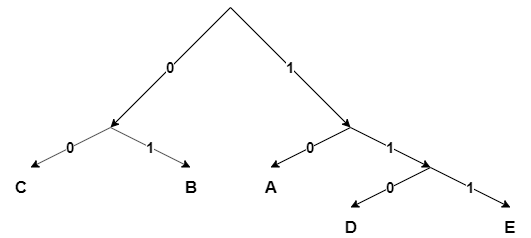
\includegraphics[width=0.6\textwidth]{img/shannon_code_tree.png}
    \caption{Shannon-kód példa 2. kódfája}
    \label{fig:shannon_code_tree}
    \end{figure}

    \noindent \textbf{Huffman kód előállítás:}

    \begin{enumerate}
        \item Az üzenetekben előforduló szimbólumok előfordulási gyakoriságának meghatározása.
        \item A szimbólumok gyakoriság szerinti csökkenő sorrendbe rendezése.
        \item A két legkevésbé gyakori szimbólumot összevonjuk és  beírjuk a szimbólumok közé a gyakorisági sorba.
        \item A 3.-ik pontot addig ismételjük, amíg 2 elemű lesz a lista.  Ekkor az egyik elemhez 0-át a másikhoz 1-et rendelünk.
        \item Visszalépünk az előző összevont szimbólumhoz, és az  előbbivel azonos sorrendben a két szimbólumhoz 0-át és 1-et rendelünk, mindaddig, míg vissza nem jutunk az egyes szimbólumokhoz.\\
    \end{enumerate}

    \noindent \emph{Példa 2}:\\

    \renewcommand{\arraystretch}{1.4}
    {\footnotesize
        \noindent \begin{tabular}{|l|l|l|l|l|}
            \hline
            % after \\: \hline or \cline{col1-col2} \cline{col3-col4} ...
            \textbf{Szimbólumok} & \textbf{Gyakoriság} & \textbf{Relatív gyakoriság} & \textbf{Információ tartalom} & \textbf{Bitek száma} \\ \hline
            A       & 6      & $\ddfrac{6}{39} \simeq 0.15$ & $-log_{2}(\ddfrac{6}{39}) = 2.70$  & $-log_2(\ddfrac{6}{39}) * 6 = 16.20$ \\ \hline
            B       & 7      & $\ddfrac{7}{39} \simeq 0.17$ & $-log_{2}(\ddfrac{7}{39}) = 2.47$  & $-log_2(\ddfrac{7}{39}) * 7 = 17.34$ \\ \hline
            C       & 15     & $\ddfrac{15}{39} \simeq 0.38$ & $-log_{2}(\ddfrac{15}{39}) = 1.37$ & $-log_2(\ddfrac{15}{39}) * 15 = 20.67$ \\ \hline
            D       & 6      & $\ddfrac{6}{39} \simeq 0.15$ & $-log_{2}(\ddfrac{6}{39}) = 2.70$  & $-log_2(\ddfrac{6}{39}) * 6 = 16.20$ \\ \hline
            E       & 5      & $\ddfrac{5}{39} \simeq 0.13$ & $-log_{2}(\ddfrac{5}{39}) = 2.96$  & $-log_2(\ddfrac{5}{39}) * 5 = 14.81$ \\ \hline
        \end{tabular}
    }
    \renewcommand{\arraystretch}{1}\\

    \noindent Rendezzük a szimbólumokat gyakoriság szerint csökkenő sorrendben:\\

    \renewcommand{\arraystretch}{1.4}
    {\footnotesize
        \noindent \begin{tabular}{|l|l|l|l|l|}
            \hline
            % after \\: \hline or \cline{col1-col2} \cline{col3-col4} ...
            \textbf{Szimbólumok} & \textbf{Gyakoriság} & \textbf{Relatív gyakoriság} & \textbf{Információ tartalom} & \textbf{Bitek száma} \\ \hline
            C       & 15     & $\ddfrac{15}{39} \simeq 0.38$ & $-log_{2}(\ddfrac{15}{39}) = 1.37$ & $-log_2(\ddfrac{15}{39}) * 15 = 20.67$ \\ \hline
            B       & 7      & $\ddfrac{7}{39} \simeq 0.17$ & $-log_{2}(\ddfrac{7}{39}) = 2.47$  & $-log_2(\ddfrac{7}{39}) * 7 = 17.34$ \\ \hline
            A       & 6      & $\ddfrac{6}{39} \simeq 0.15$ & $-log_{2}(\ddfrac{6}{39}) = 2.70$  & $-log_2(\ddfrac{6}{39}) * 6 = 16.20$ \\ \hline
            D       & 6      & $\ddfrac{6}{39} \simeq 0.15$ & $-log_{2}(\ddfrac{6}{39}) = 2.70$  & $-log_2(\ddfrac{6}{39}) * 6 = 16.20$ \\ \hline
            E       & 5      & $\ddfrac{5}{39} \simeq 0.13$ & $-log_{2}(\ddfrac{5}{39}) = 2.96$  & $-log_2(\ddfrac{5}{39}) * 5 = 14.81$ \\ \hline
        \end{tabular}\\\\
    }
    \renewcommand{\arraystretch}{1}

    \renewcommand{\arraystretch}{1.8}
    {\footnotesize
        \noindent \begin{tabular}{|llllllllllll|}
            \hline
            {\color[HTML]{333333} Szimbólumok}    &    &            &                 &        &            &               &        &            &           &          &           \\ \hline
            C             & 15 & \multicolumn{1}{l|}{}          & {\color[HTML]{333333} C}            & {\color[HTML]{333333} 15}      & \multicolumn{1}{l|}{}          & C             & 15         & \multicolumn{1}{l|}{}          & {\color[HTML]{00009B} \textit{\textbf{ABDE}}} & {\color[HTML]{333333} 24}    & {\color[HTML]{9A0000} \textbf{1}} \\ \cline{7-7}
            B             & 7  & \multicolumn{1}{l|}{}          & {\color[HTML]{010066} \textit{\textbf{DE}}}         & {\color[HTML]{333333} \textbf{11}} & \multicolumn{1}{l|}{}          & \multicolumn{1}{l|}{\cellcolor[HTML]{FFFFC7}{\color[HTML]{303498} {\ul \textbf{AB}}}} & {\color[HTML]{303498} \textbf{13}} & \multicolumn{1}{l|}{{\color[HTML]{9A0000} \textbf{1}}} & {\color[HTML]{333333} C}      & {\color[HTML]{333333} 15}    & {\color[HTML]{9A0000} \textbf{0}} \\ \cline{4-4}
            A             & 6  & \multicolumn{1}{l|}{}          & \multicolumn{1}{l|}{\cellcolor[HTML]{FFFFC7}{\color[HTML]{333333} {\ul B}}} & {\color[HTML]{333333} \textbf{7}}  & \multicolumn{1}{l|}{{\color[HTML]{9A0000} \textbf{1}}} & \multicolumn{1}{l|}{\cellcolor[HTML]{FFFFC7}{\color[HTML]{333333} {\ul DE}}}      & {\color[HTML]{333333} 11}      & \multicolumn{1}{l|}{{\color[HTML]{9A0000} \textbf{0}}} & {\color[HTML]{00009B} \textit{\textbf{}}}     & {\color[HTML]{CB0000} \textbf{}} &           \\ \cline{1-1} \cline{7-7}
            \multicolumn{1}{|l|}{\cellcolor[HTML]{FFFFC7}{\ul D}} & 6  & \multicolumn{1}{l|}{{\color[HTML]{9A0000} \textbf{1}}} & \multicolumn{1}{l|}{\cellcolor[HTML]{FFFFC7}{\ul A}}    & 6          & \multicolumn{1}{l|}{{\color[HTML]{9A0000} \textbf{0}}} &               &        & \multicolumn{1}{l|}{}          & {\color[HTML]{00009B} \textit{\textbf{}}}     & {\color[HTML]{CB0000} \textbf{}} &           \\ \cline{4-4}
            \multicolumn{1}{|l|}{\cellcolor[HTML]{FFFFC7}{\ul E}} & 5  & \multicolumn{1}{l|}{{\color[HTML]{9A0000} \textbf{0}}} &                 &        & \multicolumn{1}{l|}{}          &               &        & \multicolumn{1}{l|}{}          &           &          &           \\ \hline
        \end{tabular}\\\\
    }
    \renewcommand{\arraystretch}{1}

    \noindent $\begin{array}{c|c|c|c|c}
        \textbf{C} & \textbf{B} & \textbf{A} & \textbf{D} & \textbf{E} \\
        {\color[HTML]{CB0000} \textbf{0}} & {\color[HTML]{CB0000} \textbf{111}} & {\color[HTML]{CB0000} \textbf{110}} & {\color[HTML]{CB0000} \textbf{101}} & {\color[HTML]{CB0000} \textbf{100}} \\
        & \text{ABDE} \rightarrow \text{AB} \rightarrow \text{B} & \text{ABDE} \rightarrow \text{AB} \rightarrow \text{A} & \text{ABDE} \rightarrow \text{DE} \rightarrow \text{D} & \text{ABDE} \rightarrow \text{DE} \rightarrow \text{E} \\
    \end{array}$\\\\

    \noindent A kódfát \ref{fig:huffman_code_tree}. ábrán láthatjuk.\\

    \begin{figure}[H]
        \centering
        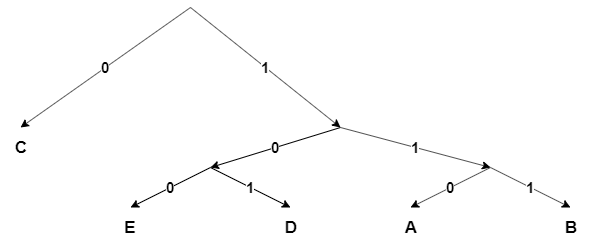
\includegraphics[width=0.65\textwidth]{img/huffman_code_tree.png}
        \caption{Huffman-kód példa 2. kódfája}
        \label{fig:huffman_code_tree}
    \end{figure}
			
\subsection*{Hibajavító kódok, kódtávolság\\}
			
    \paragraph*{Hibakorlátozó kódolás\\}

    A hibakorlátozó kódokat két csoportba sorolhatjuk: \emph{hibajelző} és \emph{hibajavító} kódok. \\
    Mindkét esetben az üzenetekhez kódszavakat rendelünk, amik alapján az átvitel során keletkező hibákat kezelni tudjuk.\\

    \noindent Amennyiben az üzenet
    \begin{itemize}[leftmargin=5.5mm]
        \renewcommand{\labelitemi}{$\vcenter{\hbox{\tiny$\bullet$}}$}
        \item \emph{könnyen ismételhető} $\Longrightarrow$ \emph{\textbf{hibajelző}},
        \item \emph{nehezen ismételhető} $\Longrightarrow$ \emph{\textbf{hibajavító}} kódot alkalmazunk.
    \end{itemize}

    \paragraph*{Kódok távolsága, súlya\\}

    A kódábécé $u$ és $v$ szavának \emph{\textbf{Hamming-távolsága}} $d(u,v)$ az azonos pozícióban levő, eltérő jegyek száma. \\
\newpage
    \noindent A Hamming-távolság rendelkezik a távolság szokásos tulajdonságaival, vagyis $\forall u,v,z$:
    \begin{itemize}[leftmargin=5.5mm]
        \renewcommand{\labelitemi}{$\vcenter{\hbox{\tiny$\bullet$}}$}
        \item $d(u,v) \geq 0$
        \item $d(u,v) = 0 \ \Longleftrightarrow \ u = v$
        \item $d(u,v) = d(v,u) \qquad $ (szimmetria)
        \item $d(u,z) \leq d(u,v)+d(v,z) \qquad$ (háromszög egyenlőtlenség)
    \end{itemize}

    \noindent \textbf{A kód távolsága}
    \[
        d(C) = \min\limits_{u\neq v}d(u,v) \qquad (u,v \in C)
    \]

    \noindent Amennyiben az $A$ kódábécé Abel-csoport a $0$ nullelemmel, ekkor egy $u$ szó \emph{\textbf{Hamming-súlya}} $w(u)$ a szóban szereplő nem nulla elemek száma. \\
    Ekkor a kód súlya
    \[
        w(C)  = \min\limits_{u\neq 0}w(u)
    \]

    \paragraph*{Hibajavító kód}

    Amikor egy olyan szót kapunk, ami nem kódszó, a hozzá legkisebb Hamming-távolságú kódszóra javítjuk.

    \begin{itemize}[leftmargin=5.5mm]
        \renewcommand{\labelitemi}{$\vcenter{\hbox{\tiny$\bullet$}}$}
        \item A $K$ kód \emph{\textbf{t-hibajavító}}, ha egy legfeljebb $t$ helyen megváltozott kódot helyesen javít.
        \item A $K$ kód \emph{\textbf{pontosan t-hibajavító}}, ha $t$-hibajavító, de nem $t+1$-hibajavító.
    \end{itemize}

    \noindent \textit{Megjegyzés}: d minimális távolságú kód esetén $\ddfrac{d}{2}$-nél kevesebb hibát biztosan egyértelműen tudunk javítani.

    \paragraph*{Hamming-korlát\\}

    Egy $q$ elemű ábécé $n$ hosszú szavaiból álló $C$ kód $t$-hibajavító. \\
    Ekkor bármely két kódszóra a tőlünk legfeljebb $t$ távolságra lévő szavak halmazai diszjunktak.\\

    \noindent Mivel egy kódszótól $j$ távolságra pontosan $\binom{n}{j}(q-1)^j$ szó van, így a \emph{\textbf{Hamming-korlát}} a kódszavak számára adott $t$-nél:
    \[\#(C) \cdot \sum\limits_{j=0}^{t}\binom{n}{j}(q-1)^j \leq q^n \]

    \noindent Amennyiben egyenlőség áll fent \emph{tökéletes kód}ról beszélünk.

    \subsection*{Lineáris kódok}
			
    $A$ véges test és $A^n$ lineáris tér. Minden $ K \leq A^n$ alteret \emph{\textbf{lineáris kód}}nak nevezzük. \\
    Ha az altér
    \begin{itemize}[leftmargin=5.5mm]
        \renewcommand{\labelitemi}{$\vcenter{\hbox{\tiny$\bullet$}}$}
        \item $k$ dimenziós,
        \item a kód távolsága $d$ és
        \item $\#(A) = q$ (\emph{Hamming-korlát})
    \end{itemize}
    akkor az ilyen kódot $[n,k,d]_q$ kódnak nevezzük.\\

    \noindent Egy lineáris kódnál feltesszük, hogy kódolandó üzenetek $K^k$ elemei, azaz a kódábécé elemeiből képzett $k$-asok.

    \paragraph*{Generátormátrix}

    $K$ véges test feletti $[n,k,d]_q$ lineáris kódolást válasszuk egy (kölcsönösen egyértelmű) lineáris leképezésnek:
    \[
        G:K^k \rightarrow K^n
    \]
    Ezt egy mátrixszal, az úgy nevezett generátormátrixszal jellemezhetjük.

    \paragraph*{Polinomkódok}

    Egy lineáris kód esetén az üzeneteket megfeleltethetjük $\mathbb{F}_q$ ($q$ elemű véges test) feletti $k$-nál alacsonyabb fokú polinomoknak.
    \[
        (a_0,a_1,\cdots,a_{k-1}) \rightarrow a_0+a_1x+\cdots+a_{k-1}x^{k-1}
    \]\\

    \noindent Legyen $G(x)$ rögzített $m$-edfokú polinom. A $p(x)$ polinomot (üzenet) $G(x)$-szel szorozva lineáris kódolást kapunk (mivel a $p \rightarrow pG$ kölcsönösen egyértelmű).\\

    \noindent Ekkor a kódszavak hossza: $n=k+m$. \\

    \noindent Az ilyen típusú lineáris kódolást \emph{\textbf{polinomkódolás}}nak nevezzük.\\

    {\footnotesize \noindent \textit{Megjegyzés}: Feltehetjük, hogy $G(x)$ főpolinom (együtthatója egység), illetve a konstans tag nem nulla (ha nulla lenne, a szorzatban kiesne a konstans tag, így a kódban a nulla indexű betű soha nem hordozna információt)}

    \paragraph*{CRC - Cyclic Redundancy Check\\}

    Ha egy polinomkódban $G(x) \big| x^n-1$, akkor \emph{\textbf{ciklikus kód}}ról beszélünk.\\

    \noindent Ekkor, ha $a_0a_1\cdots a_{\textbf{n-1}}$ kódszó, akkor $a_{\textbf{n-1}}a_0\cdots a_{n-2}$ is az, mivel:
    \[
        a_{n-1}+a_0x+\cdots+a_{n-2}x^{n-1} \ = \ x\cdot(a_0+a_1x+\cdots a_{n-1}x^{n-1})-a_{n-1}(x^n-1)
    \]
    osztható $G(x)$-szel.\\

    \noindent A \emph{CRC} az $\mathbb{F}_2$ feletti ciklikus kódokat foglalja magába, és \emph{kizárólag hibajelzésre alkalmas}. \\

    \noindent A kódolás menete következő:
    \begin{enumerate}
        \item Vegyük $p(x)x^m = (0,\ 0,\ \cdots\ ,\ 0,\ a_m,\ a_{m+1},\ \cdots\ ,\ a_{n-1})$
        \item Ezt osszuk el $G(x)$-el maradékosan
        \begin{center}
            $p(x)x^m = q(x)G(x)+r(x)$
        \end{center}
    \end{enumerate}
    Ekkor a kódszó legyen:
    \[
        p(x)x^m-r(x) = q(x)G(x)
    \]
    Ez osztható $G(x)$-szel és magas fokszámokon az eredeti üzenet betűi helyezkednek el.\\

    \noindent A fogadott szó ellenőrzése: Megnézzük, hogy osztható-e $G(x)$-szel. Ha nem oszható, akkor hiba történt.\\

\newpage

    \subsection*{Kiegészítés}

    \paragraph*{Shannon-kód}

    A következő módon állítjuk elő:
    \begin{enumerate}
        \item Rendezzük a betűket relatív gyakoriságaik alapján csökkenő sorrendbe.
        \item Határozzuk meg az $l_1,\cdots,l_n$ szóhosszúságokat a következő módon:
        \[r^{-l_i} \leq p_i < r^{-l_i+1} \]
        \item Osszuk el az ábécé elemeit az egyes helyiértékeken.\\
    \end{enumerate}

    \noindent \emph{Példa 1}:\\

    \noindent Legyen a kódábécé a ${0,1,2}$ halmaz, az kódolandó betűk és gyakoriságaik pedig a következők:\\

    \begin{tabular}{|c|c|c|c|c|c|c|c|c|c|}
        \hline a & b & c & d & e & f & g & h & i & j \\
        \hline 0,17 & 0,02 & 0,13 & 0,02 & 0,01 & 0,31 & 0,02 & 0,17 & 0,06 & 0,09 \\
        \hline
    \end{tabular}\\\\

    \noindent A relatív gyakoriságok rendezése után:\\

    \begin{tabular}{|c|c|c|c|c|c|c|c|c|c|}
        \hline f & a & h & c & j & i & b & d & g & e \\
        \hline 0,31 & 0,17 & 0,17 & 0,13 & 0,09 & 0,06 & 0,02 & 0,02 & 0,02 & 0,01 \\
        \hline
    \end{tabular}\\\\

    \noindent Határozzuk meg szóhosszúságokat. Az f, a, h és c esetében: $3^{-2} = r^{-l_i} \leq p_i < r^{-l_i+1} = 3^{-1} $ Tehát azok szóhosszúsága 2. A többi esetben is így járunk el:\\

    \begin{tabular}{|c|c|c|c|c|c|c|c|c|c|}
        \hline f & a & h & c & j & i & b & d & g & e \\
        \hline 0,31 & 0,17 & 0,17 & 0,13 & 0,09 & 0,06 & 0,02 & 0,02 & 0,02 & 0,01 \\
        \hline 2 & 2 & 2 & 2 & 3 & 3 & 4 & 4 & 4  & 5 \\
        \hline
    \end{tabular}\\\\

    \noindent Ezek alapján f kódszava a 00, a kódszava a 01, h-hoz a 02 tartozik, míg c-hez 10. A j-hez ezek után 11 tartozna, de mivel az 3 hosszú, így 110.\\

    \noindent A kódszavak tehát a következőképp alakulnak:\\

    \begin{tabular}{|c|c|c|c|c|c|c|c|c|c|}
        \hline f & a & h & c & j & i & b & d & g & e \\
        \hline 0,31 & 0,17 & 0,17 & 0,13 & 0,09 & 0,06 & 0,02 & 0,02 & 0,02 & 0,01 \\
        \hline 2 & 2 & 2 & 2 & 3 & 3 & 4 & 4 & 4  & 5 \\
        \hline 00 & 01 & 02 & 10 & 110 & 111 & 1120 & 1121 & 1122 & 12000 \\
        \hline
    \end{tabular} \\\\

    \noindent Az elkészült kódfa \ref{fig:shannon}. ábrán látható.

    \begin{figure}[H]
        \centering
        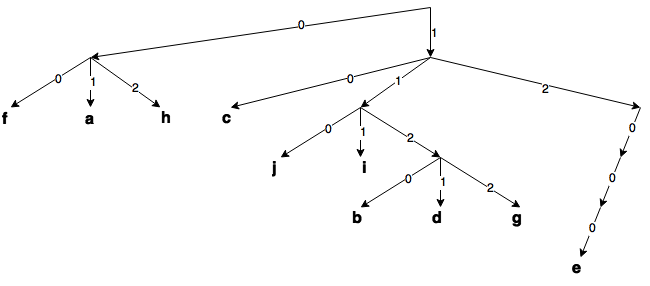
\includegraphics[width=0.6\textwidth]{img/shannon.png}
        \caption{Shannon-kód példa 1. kódfája}
        \label{fig:shannon}
    \end{figure}

    \subsection*{Hufmann-kód}

    A Huffman-kód is optimális kód ($r$ elemszámú ábécével és $p_i$ gyakoriságokkal), melyet a következő módon állítunk elő.
    \begin{enumerate}
        \item Rendezzük a betűket relatív gyakoriságaik alapján csökkenő sorrendbe.
        \item Annak érdekében, hogy csak egy csonka csúcs keletkezzen
        \[m \equiv n \mod{r-1}\]
        kongruenciának teljesülnie kell, ahol $m$ az egyetlen csonka csúcs kifoka. Ami ekvivalens azzal, hogy $m = 2 + ((n-2) \mod{r-1})$. Tehát osszuk el $n-2$-t $r-1$-gyel, és így $m$ a maradék+2 lesz.
        \item Az első lépésben a sorozat $m$ utolsó betűjét összevonjuk (új jelölést/betűt adunk neki), és ennek a relatív gyakorisága a tagok relatív gyakoriságának összege lesz. Rendezzük a sorozatot. Ezen lépés után már a betűk száma kongruens $r-1$-gyel, így a következő redukciós lépésekben mindig teljes csúcsokat tudunk készíteni.
        \item \label{itm:huffman_red} Az utolsó $r$ betűt vonjunk össze, helyettesítsük egy új betűvel és relatív gyakoriság legyen a relatív gyakoriságok összege.
        \item A \ref{itm:huffman_red}-es redukciós lépést addig ismételjük míg $r$ db betű nem marad. Ekkor rendre minden betűhöz a kódábécé egy-egy betűjét rendeljük.
        \item \label{itm:huffman_split} Ha redukált elemmel találkozunk szétbontjuk, majd az ő elemeihez is a kódábécé betűit rendeljük, de konkatenáljuk az előzővel.
        \item A \ref{itm:huffman_split}-os lépést addig ismételjük míg marad redukált elem.\\
    \end{enumerate}

    \noindent \emph{Példa 1}:\\

    \noindent A Shannon-kódnál látott forrást kódoljuk be ugyanúgy $\{0,1,2\}$ kódábécével.\\

    \noindent \begin{tabular}{|c|c|c|c|c|c|c|c|c|c|}
        \hline a & b & c & d & e & f & g & h & i & j \\
        \hline 0,17 & 0,02 & 0,13 & 0,02 & 0,01 & 0,31 & 0,02 & 0,17 & 0,06 & 0,09 \\
        \hline
    \end{tabular}\\\\
\newpage
    \noindent Rendezzük relatív gyakoriság szerint:\\

    \noindent \begin{tabular}{|c|c|c|c|c|c|c|c|c|c|}
        \hline f & a & h & c & j & i & b & d & g & e \\
        \hline 0,31 & 0,17 & 0,17 & 0,13 & 0,09 & 0,06 & 0,02 & 0,02 & 0,02 & 0,01 \\
        \hline
    \end{tabular}\\\\

    \noindent Osszuk el $n-2$-t $r-1$-gyel: $10-2 = 4*(3-1)+0$. Így $m$ a maradék+2, azaz $m=2$.\\
    Az utolsó $m$ betűt összevonjuk, és rendezzük a sorozatot:\\

    \noindent \begin{tabular}{|c|c|c|c|c|c|c|c|c|}
        \hline f & a & h & c & j & i & (g,e) & b & d  \\
        \hline 0,31 & 0,17 & 0,17 & 0,13 & 0,09 & 0,06 & 0,03 & 0,02 & 0,02 \\
        \hline
    \end{tabular}\\\\

    \noindent Innentől kezdve minden redukciós lépésben az utolsó $r$ db azaz 3 betűt vonjuk össze:\\

    \noindent \begin{tabular}{|c|c|c|c|c|c|c|}
        \hline f & a & h & c & j & ((g,e), b, d) & i  \\
        \hline 0,31 & 0,17 & 0,17 & 0,13 & 0,09 & 0,07 & 0,06  \\
        \hline
    \end{tabular}\\\\

    \noindent Ezt addig ismételjük, míg $r$ darab betű marad:\\

    \noindent \begin{tabular}{|c|c|c|}
        \hline (a,h,c) & f & (j,((g,e),b,d),i) \\
        \hline 0,47 & 0,31 & 0,22 \\
        \hline
    \end{tabular}\\\\

    \noindent A szétbontás alapján a \ref{fig:huffmann_split}. ábrán látható fát tudjuk összeállítani.\\

    \begin{figure}[H]
        \centering
        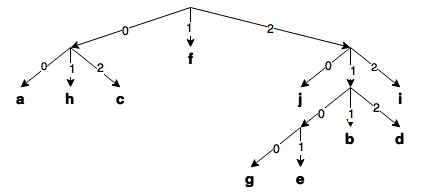
\includegraphics[width=0.65\textwidth]{img/huffmann_split.png}
        \caption{Huffman-kód példa 1. kódfája}
        \label{fig:huffmann_split}
    \end{figure}

    \noindent Ezek alapján a kódtábla:\\

    \noindent \begin{tabular}{|c|c|c|}
        \hline betű & gyakoriság & kód \\
        \hline f & 0,31 & 1 \\
        \hline a & 0,17 & 00\\
        \hline h & 0,17 & 01\\
        \hline c & 0,13 & 02\\
        \hline j & 0,09 & 20\\
        \hline i & 0,06 & 22\\
        \hline b & 0,02 & 211\\
        \hline d & 0,02 & 212\\
        \hline g & 0,02 & 2100\\
        \hline e & 0,01 & 2101\\
        \hline
    \end{tabular}
			
\end{document} 